\subsection{\texorpdfstring{\(C_{l}\) 型系统 (\(l \geqslant 2\))}{C\_l 型系统 (l >= 2)}}

\begin{enumerate}
\def\labelenumi{(\Roman{enumi})}
\item
  \(C_{l}\) 型根系的存在已在第 5 号中得到证明，因为我们已经看到，\(B_{l}\) 型系统的逆系统是 \(C_{l}\) 型。因此，一个 \(C_{l}\) 型根系可由在 \(R^{l}\) 中取向量 \(\pm2\varepsilon_{i}\ (1\leqslant i\leqslant l)\) 和 \(\pm\varepsilon_{i}\pm\varepsilon_{j}\ (1\leqslant i<j\leqslant l)\) 得到。根的数目为 \(2l^{2}\)。
\item
  对第 5 号中所考察系统的基应用映射 \(\alpha\mapsto\frac{2\alpha}{(\alpha|\alpha)}\) 所得的像，可以作为 R 的一个基。我们得到：
\end{enumerate}

\[
\alpha_ {1} = \varepsilon_ {1} - \varepsilon_ {2}, \alpha_ {2} = \varepsilon_ {2} - \varepsilon_ {3}, \dots , \alpha_ {l - 1} = \varepsilon_ {l - 1} - \varepsilon_ {l}, \alpha_ {l} = 2 \varepsilon_ {l}.
\]

正根是 \(2\varepsilon_{i}\) 以及 \(\varepsilon_{i} \pm \varepsilon_{j} (i < j)\)。

\begin{enumerate}
\def\labelenumi{(\Roman{enumi})}
\setcounter{enumi}{2}
\item
  Coxeter 数与逆系统的相同：\(h = 2l\)。
\item
  令 \(\tilde{\alpha}=2\varepsilon_{1}=2\alpha_{1}+2\alpha_{2}+\cdots+2\alpha_{l-1}+\alpha_{l}\)，这是一个根。相对于 \((\alpha_{i})\)，它的坐标之和为 2l-1=h-1。因此，\(\tilde{\alpha}\) 是最高根。我们有 \((\tilde{\alpha}|\alpha_{i})=0\)（当 \(i\neq l\) 时），\((\tilde{\alpha}|\alpha_{l})=2\)。从而，扩展 Dynkin 图为
\end{enumerate}

\[
\alpha_ {1} \quad \alpha_ {2} \quad \dots \quad \alpha_ {l - 2} \quad \alpha_ {l - 1} \quad \alpha_ {l}
\]

\begin{enumerate}
\def\labelenumi{(\Alph{enumi})}
\setcounter{enumi}{21}
\tightlist
\item
  我们已经确定了 \(R^{-}\)，它是 \(B_{l}\) 型的。由 § 1 第 12 号的公式 (19) 及第 5 号 (V)，\(2\varepsilon_{i}\) 在 \(\Phi_{R}\) 下的长度平方为
\end{enumerate}

\[
((l + 1) (4 l - 2)) ^ {+ 1} ((4 l - 2) ^ {- 1}) ^ {- 1} = (l + 1) ^ {- 1};
\]

从而，\(\Phi_{\mathrm{R}}(x,y) = (x|y) / 4(l + 1)\)。

我们有 \(\gamma(R) = \gamma(R') = (l + 1)(4l - 2)\)。

\begin{enumerate}
\def\labelenumi{(\Roman{enumi})}
\setcounter{enumi}{5}
\tightlist
\item
  基本权容易求得：
\end{enumerate}

\[
\begin{array}{l} \omega_ {i} = \varepsilon_ {1} + \varepsilon_ {2} + \dots + \varepsilon_ {i} \\ = \alpha_ {1} + 2 \alpha_ {2} + \dots + (i - 1) \alpha_ {i - 1} + i (\alpha_ {i} + \alpha_ {i + 1} + \dots + \frac {1}{2} \alpha_ {l}) (i \leqslant l). \end{array}
\]

\begin{enumerate}
\def\labelenumi{(\Roman{enumi})}
\setcounter{enumi}{6}
\tightlist
\item
  正根之和为
\end{enumerate}

\[
\begin{array}{r l} 2 \rho & = 2 l \varepsilon_ {1} + (2 l - 2) \varepsilon_ {2} + \dots + 4 \varepsilon_ {l - 1} + 2 \varepsilon_ {l} \\ & = 2 l \alpha_ {1} + 2 (2 l - 1) \alpha_ {3} + \dots + i (2 l - i + 1) \alpha_ {i} + \dots \\ & \qquad \dots + (l - 1) (l + 2) \alpha_ {l - 1} + \frac {1}{2} l (l + 1) \alpha_ {l}. \end{array}
\]

\begin{enumerate}
\def\labelenumi{(\Roman{enumi})}
\setcounter{enumi}{7}
\item
  根据第 4 号和第 5 号 (VIII)，\(Q(R) = L_{1}\)，\(P(R) = L_{0}\)；\(P(R)/Q(R)\) 同构于 Z/2Z，连接指标为 2。
\item
  以及 (X) 这些数据只取决于 W(R)，因此与 \(B_{l}\) 型的相同。
\item
  与第 5 号中相同的论证表明 \(A(R) = W(R)\) 且 \(w_0 = -1\)。
\item
  \(\mathrm{P}(\mathrm{R}^{-})/\mathrm{Q}(\mathrm{R}^{-})\) 的唯一非单位元定义了扩展 Dynkin 图的唯一非平凡自同构：它把对应于 \(\alpha_{j}\) 和 \(\alpha_{l-j}\)（\(0 \leqslant j \leqslant l\)）的顶点互换。
\end{enumerate}

\subsection{\texorpdfstring{\(\mathbf{A}_l\) 型系统 (\(l \geqslant 1\))}{A\_l 型系统 (l >= 1)}}

\begin{enumerate}
\def\labelenumi{(\Roman{enumi})}
\tightlist
\item
以及 (II) 设 \(V\) 是 \(E = R^{l + 1}\) 中方程为 \(\sum_{i=1}^{l + 1} \xi_i = 0\) 的超平面。将第 5 号中的 \(l\) 换成 \(l + 1\)，我们得到一个 \(R'\) 的 \(B_{l + 1}\) 型系统，它位于 \(E\) 中，其基为
\end{enumerate}

\[
\alpha_ {1} = \varepsilon_ {1} - \varepsilon_ {2}, \alpha_ {2} = \varepsilon_ {2} - \varepsilon_ {3}, \dots , \alpha_ {l} = \varepsilon_ {l} - \varepsilon_ {l + 1}. \alpha_ {l + 1} = \varepsilon_ {l + 1}.
\]

由于 \(\alpha_{1},\ldots,\alpha_{l}\) 生成 V，\(R=R^{\prime}\cap V\) 是 V 中以 \((\alpha_{1},\ldots,\alpha_{l})\) 为基的根系（§ 1，第 7 号，命题 20 的推论 4）。根据第 5 号中的标量积计算，立即可知 R 是 \(A_{l}\) 型的。R 的元素是 \(\varepsilon_{i}-\varepsilon_{j}\)（\(i\neq j,1\leqslant i\leqslant l+1,1\leqslant j\leqslant l+1\)）。根的数目为 \(n=l(l+1)\)。正根是 \(\varepsilon_{i}-\varepsilon_{j}\)，其中 \(i<j\)。

\begin{enumerate}
\def\labelenumi{(\Roman{enumi})}
\setcounter{enumi}{2}
\item
  我们有 \(h = n / l = l + 1\)。
\item
  令 \(\tilde{\alpha} = \varepsilon_1 - \varepsilon_{l+1} = \alpha_1 + \alpha_2 + \cdots + \alpha_l\)，这是一个根。相对于 \((\alpha_i)\)，它的坐标之和为 \(l = h - 1\)。因此，\(\tilde{\alpha}\) 是最高根。
\end{enumerate}

当 \(l = 1\) 时，\(\tilde{\alpha} = \alpha_{1}\)，所以 \((\tilde{\alpha}|\alpha_{1}) = 2\)；群 \(W_{a}(R)\) 的 Coxeter 图为

当 \(l \geqslant 2\) 时，\((\tilde{\alpha}|\alpha_i) = 0\) 对 \(0 < i < l\) 成立，且 \((\tilde{\alpha}|\alpha_1) = (\tilde{\alpha}|\alpha_l) = 1\)。因此，扩展 Dynkin 图为：

\pandocbounded{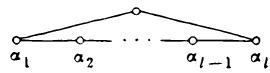
\includegraphics[keepaspectratio]{images/part002_36cfe44b.jpg}}

\begin{enumerate}
\def\labelenumi{(\Alph{enumi})}
\setcounter{enumi}{21}
\tightlist
\item
利用标量积将 V 与其对偶识别，我们有 \(\alpha^{\prime} = \frac{2\alpha}{(\alpha|\alpha)} = \alpha\) 对所有 \(\alpha \in R\) 成立，所以 \(R^{\prime} = R\)。
\end{enumerate}

对于形式 \(\Phi_{\mathbb{R}}\)，根的长度为 \(h^{-1/2} = (l + 1)^{-1/2}\)（§ 1，第 12 号）；因此 \(\Phi_{\mathrm{R}}(x,y) = (x|y)/2(l+1)\)。

我们有 \(\gamma (\mathbb{R}) = (l + 1)^2\)（§ 1，第 12 号，公式 (20)）。

\begin{enumerate}
\def\labelenumi{(\Roman{enumi})}
\setcounter{enumi}{5}
\tightlist
\item
  令 \((\omega_{i})_{1\leqslant i\leqslant l}\) 为基本权族。置
\end{enumerate}

\[
\omega_ {i} = \sum_ {j = 1} ^ {l + 1} \xi_ {i j} \varepsilon_ {j}. \quad \text { with } \xi_ {i j} \in \mathbf {R}.
\]

条件 \((\omega_{i}|\alpha_{j}) = \delta_{ij}\) 和 \(\omega_{i}\in V\) 给出

\[
\xi_ {i i} - \xi_ {i, i + 1} = 1, \quad \xi_ {i j} - \xi_ {i, j + 1} = 0 \text {   for   } j \neq i, \quad \sum_ {j = 1} ^ {l + 1} \xi_ {i j} = 0,
\]

由此容易得到

\[
\begin{array}{r l} \omega_ {i} & = \varepsilon_ {1} + \dots + \varepsilon_ {i} - \frac {i}{l + 1} (\varepsilon_ {1} + \dots + \varepsilon_ {l + 1}) \\ & = \frac {1}{l + 1} ((l - i + 1) (\alpha_ {1} + 2 \alpha_ {2} + \dots + (i - 1) \alpha_ {i - 1}) \\ & \quad + i ((l - i + 1) \alpha_ {i} + (l - i) \alpha_ {i + 1} + \dots + \alpha_ {l})). \end{array}
\]

\begin{enumerate}
\def\labelenumi{(\Roman{enumi})}
\setcounter{enumi}{6}
\tightlist
\item
  正根之和为
\end{enumerate}

\[
\begin{array}{r l} 2 \rho & = l \varepsilon_ {1} + (l - 2) \varepsilon_ {2} + (l - 4) \varepsilon_ {3} + \dots - (l - 2) \varepsilon_ {l} - l \varepsilon_ {l + 1} \\ & = l \alpha_ {1} + 2 (l - 1) \alpha_ {2} + \dots + i (l - i + 1) \alpha_ {i} + \dots + l \alpha_ {l}. \end{array}
\]

\begin{enumerate}
\def\labelenumi{(\Roman{enumi})}
\setcounter{enumi}{7}
\tightlist
\item
  在 \(\mathbf{E} = \mathbf{R}^{l + 1}\) 中引入第 4 号的子群 \(\mathrm{L}_0\)。设 \(p\) 是 E 到 V 的正交投影。由 § 1，第 10 号，命题 28，有
\end{enumerate}

\[
\mathrm{Q} (\mathrm{R}) = \mathrm{Q} \left(\mathrm{R} ^ {\prime}\right) \cap \mathrm{V} \neq \mathrm{L} _ {0} \cap \mathrm{V}, \text { and } \mathrm{P} (\mathrm{R}) = p \left(\mathrm{P} \left(\mathrm{R} ^ {\prime}\right)\right);
\]

由于 \(R'\) 的最后一个基本权与 V 正交，我们有 \(\mathrm{P}(\mathrm{R}) = p(\mathrm{Q}(\mathrm{R}')) = p(\mathrm{L}_0)\)。因此，\(\mathrm{P}(\mathrm{R})\) 是由 \(\varepsilon_i - \varepsilon_j\) 以及 \(p(\varepsilon_1) = \varepsilon_1 \to (l + 1)^{-1} \sum_{i=1}^{l+1} \varepsilon_i\) 生成的群，所以

\[
\mathrm{P} (\mathrm{R}) = \mathrm{Q} (\mathrm{R}) + \mathbf {Z} \left(\varepsilon_ {1} - (l + 1) ^ {- 1} \sum_ {i = 1} ^ {l + 1} \varepsilon_ {i}\right).
\]

现在，\(l + 1\) 是满足 \(m > 0\) 且 \(mp(\varepsilon_1) \in Q(R)\) 的最小整数。因此，\(P(R)/Q(R)\) 同构于 \(\mathbf{Z}/(l + 1)\mathbf{Z}\)，连接指标为 \(l + 1\)。

\begin{enumerate}
\def\labelenumi{(\Roman{enumi})}
\setcounter{enumi}{8}
\tightlist
\item
  以及 (X) 对 V 的任意自同构 g，令 \(\varphi(g)\) 为将 g 延拓到 E 且保持 \(\varepsilon_{1} + \varepsilon_{2} + \cdots + \varepsilon_{l}\) 不变的自同构。若 g 是正交反射 \(s_{\varepsilon_{i} - \varepsilon_{j}}|V\)，则 \(\varphi(g)\) 等于 \(s_{\varepsilon_{i} - \varepsilon_{j}}\)；后者将 \(\varepsilon_{i}\) 与 \(\varepsilon_{j}\) 互换，并保持所有下标 k 与 i、j 不同的 \(\varepsilon_{k}\) 不变。令
\end{enumerate}

\[
X = \left\{\varepsilon_ {1}, \varepsilon_ {2}, \dots , \varepsilon_ {l + 1} \right\}.
\]

于是，\(g \mapsto \varphi(g)|_{\mathbf{X}}\) 是从 \(W(\mathbf{R})\) 到 \(\mathbf{X}\) 的对称群的同构。因此，\(W(\mathbf{R})\) 同构于对称群 \(\mathfrak{S}_{l+1}\)，其阶为 \((l+1)!\)。

对称代数 \(\mathbf{S}(\mathrm{E})\) 可与 E 上的多项式函数代数 \(\mathrm{P}(\xi_1, \xi_2, \ldots, \xi_{l+1})\) 作规范识别。令 \(\mathrm{G} = \varphi(\mathrm{W}(\mathrm{R}))\)。由上一段，\(\mathbf{S}(\mathrm{E})^{\mathrm{G}}\) 中在 G 下不变的 \(\mathbf{S}(\mathrm{E})\) 元素所成的集合就是对称多项式的集合（《代数》，第 V 章，附录 I），因而（同上）是由下列函数生成的代数

\[
s _ {i} ^ {\prime} = \sum_ {\tau \in \mathfrak {S} _ {l + 1}} \xi_ {\tau (1)} \xi_ {\tau (2)} \dots \xi_ {\tau (i)} \quad (1 \leqslant i \leqslant l + 1).
\]

代数 \(\mathbf{S}(\mathrm{V})\) 可识别为多项式函数在 \(\mathrm{V}\) 上的限制所成的代数，这些多项式函数定义在 \(\mathrm{E}\) 上。若 \(\mathrm{P} \in \mathbf{S}(\mathrm{E})^{\mathrm{G}}\)，则 \(\mathrm{P}\) 在 \(\mathrm{V}\) 上的限制显然在 \(\mathrm{W}(\mathrm{R})\) 下不变。反之，若 \(\mathrm{Q} \in \mathbf{S}(\mathrm{V})^{\mathrm{W}(\mathrm{R})}\)，则存在 \(\mathrm{P} \in \mathbf{S}(\mathrm{E})\) 延拓 \(\mathrm{Q}\)；将 \(\mathrm{P}\) 替换为 \(((l + 1)!)^{-1} \sum_{g \in \mathrm{G}} g(\mathrm{P})\)，所得多项式的限制与 \(\mathrm{P}\) 在 \(\mathrm{V}\) 上的限制相同。我们可以设 \(\mathrm{P} \in \mathbf{S}(\mathrm{E})^{\mathrm{G}}\)。因此，\(\mathbf{S}(\mathrm{V})^{\mathrm{W}(\mathrm{R})}\) 由 \(s_i = s_i'|\mathrm{V}\) 生成。现在 \(s_1 = 0\)。此外，在 \(\mathbf{R}\) 上，\(\mathbf{S}(\mathrm{V})^{\mathrm{W}(\mathrm{R})}\) 的分式域的超越次数为 \(l\)，所以 \(s_i\)（\(2 \leqslant i \leqslant l + 1\)）代数独立。由于 \(s_i\) 的次数为 \(2, 3, \ldots, l + 1\)，\(\mathrm{W}(\mathrm{R})\) 的指数为

\[
1, 2, 3, \dots , l.
\]

\begin{enumerate}
\def\labelenumi{(\Roman{enumi})}
\setcounter{enumi}{10}
\tightlist
\item
  当 \(l = 1\) 时，A(R) = W(R) = Z/2Z 且 \(w_0 = -1\)。
\end{enumerate}

当 \(l \geqslant 2\) 时，令 \(\varepsilon \in A(R)\) 为把 \(\alpha_i\) 变为 \(\alpha_{l+1-i}\) 的自同构。显然，由 \(\varepsilon\) 诱导的自同构是 Dynkin 图的唯一非平凡自同构。群 \(A(R)/W(R)\) 同构于 \(Z/2Z\)。由 (IX) 和 (X)，-1 是属于 \(A(R)\) 但不属于 \(W(R)\) 的元素，因此 \(A(R)\) 同构于 \(W(R) \times Z/2Z\)。我们有 \(w_0 = -\varepsilon\)。

\begin{enumerate}
\def\labelenumi{(\Roman{enumi})}
\setcounter{enumi}{11}
\tightlist
\item
  群 \(\mathrm{P}(\mathrm{R}^{-})/\mathrm{Q}(\mathrm{R}^{-})\) 是阶为 \(l+1\) 的循环群，并通过循环置换作用于扩充的 Dynkin 图。若 \(l\geqslant2\)，\(\mathrm{A}(\mathrm{R})/\mathrm{W}(\mathrm{R})\) 的唯一非恒等元素在 \(\mathrm{P}(\mathrm{R}^{-})/\mathrm{Q}(\mathrm{R}^{-})\) 上的作用是自同构 \(x\mapsto-x\)。
\end{enumerate}

\subsection{\texorpdfstring{\(D_{l}\) 型系统 (\(l \geqslant 3\))}{D\_l 型系统 (l >= 3)}}

\begin{enumerate}
\def\labelenumi{(\Roman{enumi})}
\item
  在 \(V = R^{l}\) 中考虑第 4 号的群 \(L_{0}\)。集合 R 中满足 \(\alpha \in L_{0}\) 且 \((\alpha|\alpha) = 2\) 的根由向量 \(\pm\varepsilon_{i} \pm \varepsilon_{j}\)（ \(1 \leqslant i < j \leqslant l\)）组成。显然，R 生成 V，且 \(2(\alpha|\beta)/(\alpha|\alpha) \in \mathbf{Z}\) 对所有 \(\alpha, \beta \in R\) 成立。因此，R 是 V 中的约化根系（第 4 号）。根的数目为 \(n = 2l(l - 1)\)。
\item
  令
\end{enumerate}

\[
\alpha_ {1} = \varepsilon_ {1} - \varepsilon_ {2}, \alpha_ {2} = \varepsilon_ {2} - \varepsilon_ {3} \dots . \alpha_ {l - 1} = \varepsilon_ {l - 1} - \varepsilon_ {l}, \alpha_ {l} = \varepsilon_ {l - 1} + \varepsilon_ {l}.
\]

下列公式是显然的：

\[
\begin{array}{c} \varepsilon_ {i} - \varepsilon_ {j} = \alpha_ {i} + \alpha_ {i + 1} + \dots + \alpha_ {j - 1} (i <   j) \\ \varepsilon_ {i} + \varepsilon_ {j} = \alpha_ {i} + \alpha_ {i + 1} + \dots + \alpha_ {j - 1} + 2 \alpha_ {j} + 2 \alpha_ {j + 1} + \dots \\ \qquad \qquad \qquad \qquad \qquad \qquad \dots + 2 \alpha_ {l - 2} + \alpha_ {l - 1} + \alpha_ {l} (i <   j \leqslant l - 2) \\ \varepsilon_ {i} + \varepsilon_ {l - 1} = \alpha_ {i} + \alpha_ {i + 1} + \dots + \alpha_ {l} (i <   l - 1) \\ \varepsilon_ {i} + \varepsilon_ {l} = \alpha_ {i} + \alpha_ {i + 1} + \dots + \alpha_ {l - 2} + \alpha_ {l} (i <   l - 1) \\ \varepsilon_ {l - 1} + \varepsilon_ {l} = \alpha_ {l}. \end{array}
\]

所以 \((\alpha_{1},\ldots,\alpha_{l})\) 是 R 的一个基（§ 1，第 2 号，命题 20 的推论 3）。此外，\(\| \alpha_{i}\|^{2}=2\) 对所有 \(i\) 成立，且 \((\alpha_{i}|\alpha_{j})=0\) 对 \(i+1<j\) 成立，但 \(i=l-2\)、\(j=l\) 时例外，此时 \((\alpha_{l-2}|\alpha_{l})=-1\)；\((\alpha_{i}|\alpha_{i+1})=-1\) 对 \(i\leqslant l-2\) 成立，最后 \((\alpha_{l-1}|\alpha_{l})=-1\)；因此 R 的 Dynkin 图为 D \(_{l}\) 型。正根是 \(\varepsilon_{i}\pm\varepsilon_{j}\)，其中 \(i<j\)。

\begin{enumerate}
\def\labelenumi{(\Roman{enumi})}
\setcounter{enumi}{2}
\item
  我们有 \(h = n / l = 2(l - 1)\)。
\item
  令 \(\tilde{\alpha} = \varepsilon_{1} + \varepsilon_{2} = \alpha_{1} + 2\alpha_{2} + \cdots + 2\alpha_{l-2} + \alpha_{l-1} + \alpha_{l}\)，这是一个根。相对于 \((\alpha_{i})\)，它的坐标之和为
\end{enumerate}

\[
2 l - 3 = h - 1.
\]

因此 \(\tilde{\alpha}\) 是最高根。

若 \(l = 3\)，则有

\[
(\tilde {\alpha} | \alpha_ {1}) = 0, \quad (\tilde {\alpha} | \alpha_ {2}) = (\tilde {\alpha} | \alpha_ {3}) = 1.
\]

若 \(l \geqslant 4\)，则 \((\tilde{\alpha}|\alpha_i) = 0\) 当 \(i \neq 2\) 时成立，且 \((\tilde{\alpha}|\alpha_2) = 1\)。因此，扩展 Dynkin 图为：

\[
\alpha_ {1} \quad \alpha_ {2} \quad \alpha_ {3} \quad \dots \quad \alpha_ {i - 3} \quad \alpha_ {i - 2} \quad \alpha_ {i - 1}
\]

\begin{enumerate}
\def\labelenumi{(\Alph{enumi})}
\setcounter{enumi}{21}
\tightlist
\item
  由于 \((\alpha |\alpha) = 2\) 对所有 \(\alpha \notin R\) 成立，所以 \(R^{\sim} = R\)。
\end{enumerate}

对于 \(\Phi_{\mathrm{R}}\)，根的长度为 \(h^{-1 / 2} = (2l - 2)^{-1 / 2}\)。因此

\[
\Phi_ {R} (x, y) = (x | y) / (4 l - 4) \quad \text { and } \quad \gamma (R) = 4 (l - 1) ^ {2}.
\]

\begin{enumerate}
\def\labelenumi{(\Roman{enumi})}
\setcounter{enumi}{5}
\tightlist
\item
  类似于第 7 号的计算给出基本权：
\end{enumerate}

\[
\begin{array}{r l} \omega_ {i} & = \varepsilon_ {1} + \varepsilon_ {2} + \dots + \varepsilon_ {i} \\ & = \alpha_ {1} + 2 \alpha_ {2} + \dots + (i - 1) \alpha_ {i - 1} + i (\alpha_ {i} + \alpha_ {i + 1} + \dots + \alpha_ {l - 2}) \\ & \quad + \frac {1}{2} i (\alpha_ {l - 1} + \alpha_ {l}) \end{array}
\]

当 i \textless{} l - 1 时，

\[
\begin{array}{l} \omega_ {l - 1} = \frac {1}{2} (\varepsilon_ {1} + \varepsilon_ {2} + \dots + \varepsilon_ {l - 2} + \varepsilon_ {l - 1} - \varepsilon_ {l}) \\ \qquad = \frac {1}{2} (\alpha_ {1} + 2 \alpha_ {2} + \dots + (l - 2) \alpha_ {l - 2} + \frac {1}{2} l \alpha_ {l - 1} + \frac {1}{2} (l - 2) \alpha_ {l}), \\ \omega_ {l} = \frac {1}{2} (\varepsilon_ {1} + \varepsilon_ {2} + \dots + \varepsilon_ {l - 2} + \varepsilon_ {l - 1} + \varepsilon_ {l}) \\ \qquad = \frac {1}{2} (\alpha_ {1} + 2 \alpha_ {2} + \dots + (l - 2) \alpha_ {l - 2} + \frac {1}{2} (l - 2) \alpha_ {l - 1} + \frac {1}{2} l \alpha_ {l}). \end{array}
\]

\begin{enumerate}
\def\labelenumi{(\Roman{enumi})}
\setcounter{enumi}{6}
\tightlist
\item
  正根之和为
\end{enumerate}

\[
\begin{array}{l} 2 \rho = 2 (l - 1) \varepsilon_ {1} + 2 (l - 2) \varepsilon_ {2} + \dots + 2 \varepsilon_ {l - 1} \\ = \sum_ {i = 1} ^ {l - 2} 2 (i l - \frac {i (i + 1)}{2}) \alpha_ {i} + \frac {l (l - 1)}{2} (\alpha_ {l - 1} + \alpha_ {l}). \end{array}
\]

\begin{enumerate}
\def\labelenumi{(\Roman{enumi})}
\setcounter{enumi}{7}
\item
  \(\pm \varepsilon_{i} \pm \varepsilon_{j}\) 生成 \(L_{1}\)（第 4 号），所以 \(Q(R) = L_{1}\)。因此 \(Q(R^{-}) = L_{1}\)，从而 \(P(R) = L_{2}\)（第 4 号）。由第 4 号，\(P(R)/Q(R)\) 同构于 \(\mathbf{Z}/4\mathbf{Z}\)（当 \(l\) 为奇数时），同构于 \(\mathbf{Z}/2\mathbf{Z} \times \mathbf{Z}/2\mathbf{Z}\)（当 \(l\) 为偶数时）。在第一种情形中，\(P(R)/Q(R)\) 由 \(\omega_{l}\) 的规范像生成（也由 \(\omega_{l-1}\) 的规范像生成）；在第二种情形中，\(P(R)/Q(R)\) 由 \(\omega_{l-1}\) 和 \(\omega_{l}\) 的规范像生成。在两种情形中，连接指标都是 4。
\item
  以及 (X) 在 \(\mathbf{R}^l\) 中，正交反射 \(s_{\varepsilon_i - \varepsilon_j}\)（ \(i \neq j\)）将 \(\varepsilon_i\) 与 \(\varepsilon_j\) 互换，并保持 \(\varepsilon_k\) 不变，其中 \(k\) 与 \(i\) 、 \(j\) 均不同。\(s_{\varepsilon_i - \varepsilon_j}\) 生成群 \(\mathbf{G}_1\)，它同构于对称群 \(\mathfrak{S}_l\)。另一方面，\(s_{ij} = s_{\varepsilon_i - \varepsilon_j} s_{\varepsilon_i + \varepsilon_j}\) 将 \(\varepsilon_i\) 变为 \(-\varepsilon_i\)，将 \(\varepsilon_j\) 变为 \(-\varepsilon_j\)，并保持 \(\varepsilon_k\) 不变，其中 \(k\) 与 \(i\) 、 \(j\) 均不同。\(s_{ij}\) 生成群 \(\mathbf{G}_2\)，它是由自同构 \(u\) 组成的 \(\mathbf{R}^l\) 的自同构群，满足 \(u(\varepsilon_i) = (-1)^{\nu_i} \varepsilon_i\) 且 \(\prod_{i=1}^{l} (-1)^{\nu_i} = 1\)。群 \(\mathbf{G}_2\) 同构于 \((\mathbf{Z}/2\mathbf{Z})^{l-1}\)，且 \(\mathbf{G}_2\) 是 W(R) 的正规子群，所以 W(R) 同构于 \(\mathfrak{S}_l\) 与 \((\mathbf{Z}/2\mathbf{Z})^{l-1}\) 的半直积。因此，其阶为 \(2^{l-1}.l!\)。
\end{enumerate}

 第 5 号的多项式函数 \(t_j\) 在 \(W(R)\) 下不变，\(t = \xi_1\xi_2\ldots\xi_l\) 也不变；此外，\(t_l = t^2\)。设 \(P(\xi_1,\ldots ,\xi_l)\) 是在 \(W(R)\) 下不变的多项式。设单项式 \(\xi_1^{\nu_1}\xi_2^{\nu_2}\ldots\xi_l^{\nu_l}\) 出现在 \(P\) 中且满足 \(\nu_{i}\) 为奇数；那么 \(\nu_{j}\) 对所有 \(j\) 都是奇数，因为单项式 \((-1)^{\nu_i + \nu_j}\xi_1^{\nu_1}\xi_2^{\nu_2}\ldots\xi_l^{\nu_l}\) 出现在 \(s_{ij}(P)\) 中，所以 \(\nu_{i} + \nu_{j} \equiv 0 \pmod{2}\)，且 \(\nu_{j} \equiv 1 \pmod{2}\)。于是

\(P = P_{1} + tP_{2}\)，其中出现在 \(P_{1}\) 和 \(P_{2}\) 中的所有单项式都只有偶数指数。由于 P 在 \(\xi_{i}\) 的置换下不变，\(P_{1}\) 和 \(P_{2}\) 也具有同样的性质，因此可以写成 \(t_{1}, t_{2}, \ldots, t_{l}\) 的多项式。这证明代数 \(\mathbf{S}(\mathbf{R}^{l})^{\mathrm{W}(\mathbb{R})}\) 由 \(t_{1}, t_{2}, \ldots, t_{l-1}, t\) 生成。此外，\(\mathbf{S}(\mathbf{R}^{l})^{\mathrm{W}(\mathbb{R})}\) 的分式域的超越次数为 l，所以 \(t_{1}, t_{2}, \ldots, t_{l-1}, t\) 代数独立。我们得到，适当排序后的指数序列为：

\[
1, 3, 5, \dots , 2 l - 5, 2 l - 3, l - 1.
\]

注意，\(l - 1\) 在 \(l\) 为偶数时出现两次，在 \(l\) 为奇数时出现一次。

\begin{enumerate}
\def\labelenumi{(\Roman{enumi})}
\setcounter{enumi}{10}
\tightlist
\item
  Dynkin 图的自同构就是其底层图的自同构。因此：
\end{enumerate}

\begin{enumerate}
\def\labelenumi{\arabic{enumi})}
\item
  若 \(l = 3\)，则 A(R)/W(R) 同构于 Z/2Z。
\item
  若 \(l = 4\)，则终端顶点的每个置换都定义图的一个自同构，所以 \(\mathrm{A}(\mathrm{R}) / \mathrm{W}(\mathrm{R})\) 同构于 \(\mathfrak{S}_3\)。
\item
  若 \(l \geqslant 5\)，则从分叉点出发的链长度为 1、1 和 \(l - 3 \geqslant 2\)。因此，除恒等自同构外，图的唯一自同构对应于自同构 \(\varepsilon \in \mathrm{A}(\mathrm{R})\)：它互换 \(\alpha_{l-1}\) 与 \(\alpha_l\)，并固定 \(\alpha_i\)（\(1 \leqslant i \leqslant l - 2\)）。于是 \(\mathrm{A}(\mathrm{R}) / \mathrm{W}(\mathrm{R})\) 同构于 \(\mathbf{Z}/2\mathbf{Z}\)；此外，\(\mathrm{A}(\mathrm{R})\) 是 (IX) 中定义的群 \(\mathbf{G}_1 \cong \mathfrak{S}_l\) 与群 \(\mathbf{G}_3\) 的半直积；该群由自同构 \(u\) 组成，这些自同构是 \(\mathbf{R}^l\) 的自同构，且 \(u(\varepsilon_i) = \pm \varepsilon_i\) 对所有 \(i\) 成立。
\end{enumerate}

若 \(l\) 为偶数，则 \(-1 \in \mathrm{W}(\mathrm{R})\)，所以 \(w_0 = -1\)。若 \(l\) 为奇数，则 \(-1 \notin \mathrm{W}(\mathrm{R})\)，所以 \(\mathrm{A}(\mathrm{R}) = \mathrm{W}(\mathrm{R}) \times \{1, -1\}\)，且 \(w_0 = -\varepsilon\)。

\begin{enumerate}
\def\labelenumi{(\Roman{enumi})}
\setcounter{enumi}{11}
\tightlist
\item
当 \(l\) 为偶数时，\(\mathrm{P}(\mathbb{R}^{-}) / \mathrm{Q}(\mathbb{R}^{-})\) 有三个 2 阶元素，即 \(\omega_{1}, \omega_{l-1}\) 和 \(\omega_{l}\)。由于 \(\omega_{l}\)（分别为 \(\omega_{l-1}\)）互换对应于 \(\alpha_{0}\) 和 \(\alpha_{l}\)（分别为 \(\alpha_{l-1}\)）的顶点，它也互换对应于 \(\alpha_{1}\) 和 \(\alpha_{l-1}\)（分别为 \(\alpha_{l}\)）的顶点，并且还互换对应于 \(\alpha_{j}\) 和 \(\alpha_{l-j}\) 的顶点，其中
\end{enumerate}

\[
2 \leqslant j \leqslant l - 2.
\]

我们有 \(\omega_{1} = \omega_{l}\omega_{l - 1}\)

当 \(l\) 为奇数时，\(\mathrm{P}(\mathbb{R}^{-}) / \mathrm{Q}(\mathbb{R}^{-})\) 有两个 4 阶元素，即 \(\omega_{l-1}\) 和 \(\omega_l\)，以及一个 2 阶元素，即 \(\omega_1\)。事实上，\(\omega_1\) 互换对应于 \(\alpha_0\) 和 \(\alpha_1\) 的顶点，所以它固定对应于 \(\alpha_j\) 的顶点，其中 \(2 \leqslant j \leqslant l-2\)，并且必为 2 阶。因此，\(\omega_l\) 是 4 阶的，并将对应于 \(\alpha_0\)（分别为 \(\alpha_l\)、\(\alpha_1\)、\(\alpha_{l-1}\)）的顶点变为对应于 \(\alpha_l\)（分别为 \(\alpha_1\)、\(\alpha_{l-1}\)、\(\alpha_0\)）的顶点，并互换对应于 \(\alpha_j\) 和 \(\alpha_{l-j}\) 的顶点，其中 \(2 \leqslant j \leqslant l-2\)。我们有 \(\omega_1 = \omega_l^2\)，且 \(\omega_{l-1} = \omega_l^3\)。

当 \(l \neq 4\) 时，\(\mathrm{A}(\mathrm{R})/\mathrm{W}(\mathrm{R})\) 的非单位元互换对应于 \(\alpha_{l-1}\) 和 \(\alpha_{l}\) 的顶点，因而互换元素 \(\omega_{l-1}\) 和 \(\omega_{l}\)（它们属于 \(\mathrm{P}(\mathrm{R}^{-})/\mathrm{Q}(\mathrm{R}^{-})\)）。当 l 为奇数时，由此得到的 \(\mathrm{P}(\mathrm{R}^{-})/\mathrm{Q}(\mathrm{R}^{-})\) 的自同构是映射 \(x \mapsto -x\)。

当 \(l = 4\) 时，\(A(R)/W(R)\) 可识别为 \(\{1,3,4\}\) 的置换群，并通过对指标的置换作用于 \(\{\omega_1,\omega_3,\omega_4\}\)。

\subsection{\texorpdfstring{\(F_{4}\) 型系统}{F\_4 型系统}}

\begin{enumerate}
\def\labelenumi{(\Roman{enumi})}
\tightlist
\item
  考虑第 4 号的群 \(\mathbf{L}_2\)，它位于 \(\mathbf{R}^4\) 中。令 \(\mathbf{R}\) 为满足 \(\alpha \in \mathbf{L}_2\) 且 \((\alpha |\alpha) = 1\) 或 \((\alpha |\alpha) = 2\) 的向量集合；它包含向量
\end{enumerate}

\[
\pm \varepsilon_ {i}, \quad \pm \varepsilon_ {i} \pm \varepsilon_ {j} (i <   j), \quad \frac {1}{2} (\pm \varepsilon_ {1} \pm \varepsilon_ {2} \pm \varepsilon_ {3} \pm \varepsilon_ {4}).
\]

反之，若 \(\alpha\in R\)，则 \(\alpha\) 的坐标只能取 \(0,\pm\frac{1}{2},\pm1\) 这些值（因为 \((\frac{3}{2})^{2}>2\)）；这些坐标要么全为整数，从而得到向量 \(\pm\varepsilon_{i},\pm\varepsilon_{i}\pm\varepsilon_{j}\)，要么全都等于 \(\pm\frac{1}{2}\)，从而得到向量 \(\frac{1}{2}(\pm\varepsilon_{1}\pm\varepsilon_{2}\pm\varepsilon_{3}\pm\varepsilon_{4})\)。

我们证明，对于 \(\alpha, \beta \in \mathbb{R}\)，有 \(2(\alpha|\beta) / (\alpha|\alpha) \in \mathbf{Z}\)。若 \(\alpha = \pm \varepsilon_i\) 或 \(\alpha = \frac{1}{2} (\pm \varepsilon_1 \pm \varepsilon_2 \pm \varepsilon_3 \pm \varepsilon_4)\)，则 \((\alpha|\alpha) = 1\)，且由第 4 号知 \((\alpha|\beta) \in \frac{1}{2}\mathbf{Z}\)，因为 \(\alpha, \beta \in \mathbf{L}_2\)。若 \(\alpha = \pm \varepsilon_i \pm \varepsilon_j\)，则 \((\alpha|\alpha) = 2\)，且由第 4 号知 \((\alpha|\beta) \in \mathbf{Z}\)，因为 \(\alpha \in \mathbf{L}_1\) 且 \(\beta \in \mathbf{L}_2\)。因此，R 是 \(\mathbf{R}^4\) 中的约化根系（第 4 号）。根的数目为 \(n = 8 + \binom{4}{2} 4 + 2^4 = 48\)。

\begin{enumerate}
\def\labelenumi{(\Roman{enumi})}
\setcounter{enumi}{1}
\tightlist
\item
  在 \(\mathbf{R}^4\) 中赋予由基 \((\varepsilon_1, \varepsilon_2, \varepsilon_3, \varepsilon_4)\) 定义的字典序（§ 1，第 7 号）。特别地，\(\varepsilon_1 > \varepsilon_2 > \varepsilon_3 > \varepsilon_4\)。正根为
\end{enumerate}

\[
\varepsilon_ {i}, \quad \varepsilon_ {i} \pm \varepsilon_ {j} (i <   j), \quad \frac {1}{2} (\varepsilon_ {1} \pm \varepsilon_ {2} \pm \varepsilon_ {3} \pm \varepsilon_ {4}).
\]

最小的根是 \(\alpha_{3} = \varepsilon_{4}\)。在属于 \(\mathbf{R}\varepsilon_{3} + \mathbf{R}\varepsilon_{4}\) 但不属于 \(\mathbf{R}\varepsilon_{4}\) 的根中，最小的是 \(\alpha_{2} = \varepsilon_{3} - \varepsilon_{4}\)。在属于 \(\mathbf{R}\varepsilon_{2} + \mathbf{R}\varepsilon_{3} + \mathbf{R}\varepsilon_{4}\) 但不属于 \(\mathbf{R}\varepsilon_{3} + \mathbf{R}\varepsilon_{4}\) 的正根中，最小的是 \(\alpha_{1} = \varepsilon_{2} - \varepsilon_{3}\)。在不属于 \(\mathbf{R}\varepsilon_{2} + \mathbf{R}\varepsilon_{3} + \mathbf{R}\varepsilon_{4}\) 的正根中，最小的是 \(\alpha_{4} = \frac{1}{2} (\varepsilon_{1} - \varepsilon_{2} - \varepsilon_{3} - \varepsilon_{4})\)。没有一个 \(\alpha_{i}\) 是两个正根之和。因此，\((\alpha_{1},\alpha_{2},\alpha_{3},\alpha_{4})\) 是 R 的一个基（§ 1，第 6 号，命题 19 的推论 1）。我们有 \(\| \alpha_1 \|^2 = \| \alpha_2 \|^2 = 2\)，\(\| \alpha_3 \|^2 = \| \alpha_4 \|^2 = 1\)，\((\alpha_1|\alpha_2) = (\alpha_2|\alpha_3) = -1\)，\((\alpha_3|\alpha_4) = -\frac{1}{2}\)，\((\alpha_1|\alpha_3) = (\alpha_1|\alpha_4) = (\alpha_2|\alpha_4) = 0\)。可见 R 的 Dynkin 图为 \(F_4\) 型，因而不可约。

\begin{enumerate}
\def\labelenumi{(\Roman{enumi})}
\setcounter{enumi}{2}
\item
  我们有 \(h = \frac{n}{l} = 12\)。
\item
  令 \(\tilde{\alpha} = \varepsilon_1 + \varepsilon_2 = 2\alpha_1 + 3\alpha_2 + 4\alpha_3 + 2\alpha_4\)。\(\tilde{\alpha}\) 相对于 \((\alpha_i)\) 的坐标之和为 \(11 = h - 1\)，所以 \(\tilde{\alpha}\) 是最高根。我们有 \((\tilde{\alpha}|\alpha_1) = 1\)，\((\tilde{\alpha}|\alpha_2) = (\tilde{\alpha}|\alpha_3) = (\tilde{\alpha}|\alpha_4) = 0\)。
\end{enumerate}

扩展 Dynkin 图为

\[
\alpha_ {1} \quad \alpha_ {2} \quad \alpha_ {3} \quad \alpha_ {4}
\]

\begin{enumerate}
\def\labelenumi{(\Alph{enumi})}
\setcounter{enumi}{21}
\tightlist
\item
  公式 \(\alpha^{\prime} = \frac{2\alpha}{(\alpha|\alpha)}\) 给出 \(R^{\prime}\) 的向量集合 \(\pm 2\varepsilon_{i}, \pm \varepsilon_{i} \pm \varepsilon_{j}, \pm \varepsilon_{1} \pm \varepsilon_{2} \pm \varepsilon_{3} \pm \varepsilon_{4}\)。\(R^{\prime}\) 的 Dynkin 图按照第 2 号所说明的步骤由 \(R\) 的 Dynkin 图得到；于是我们看到 \(R^{\prime}\) 是 \(F_{4}\) 型的。
\end{enumerate}

与 \(\beta = \varepsilon_1\) 不正交的根为 \(\pm \varepsilon_1, \pm \varepsilon_1 \pm \varepsilon_j\)（ \(j \geqslant 2\)）以及 \(\frac{1}{2} (\pm \varepsilon_1 \pm \varepsilon_2 \pm \varepsilon_3 \pm \varepsilon_4)\)；数值 \(n(\alpha | \beta) = 2(\alpha | \beta)\) 对其中前 14 个根等于 \(\pm 2\)，对后 16 个根等于 \(\pm 1\)；因此，对于 \(\Phi_R\)，\(\beta\) 的长度平方为 \(4(14.4 + 16.1)^{-1} = \frac{1}{18}\)；于是

\[
\Phi_ {R} (x, y) = \frac {(x | y)}{18}.
\]

现在对 \(x = y = \beta\) 应用 § 1 第 12 号的公式 (18)，得到

\[
2 + 12. \frac {1}{4} + 16. \frac {1 / 4}{1} = \gamma (\mathrm{R}). \frac {1}{18}
\]

所以

\[
\gamma (\mathrm{R}) = 2. 3 ^ {4}.
\]

\begin{enumerate}
\def\labelenumi{(\Roman{enumi})}
\setcounter{enumi}{5}
\tightlist
\item
  计算基本权得到
\end{enumerate}

\[
\omega_ {1} = \varepsilon_ {1} + \varepsilon_ {2} = 2 \alpha_ {1} + 3 \alpha_ {2} + 4 \alpha_ {3} + 2 \alpha_ {4} = \tilde {\alpha}
\]

\[
\omega_ {2} = 2 \varepsilon_ {1} + \varepsilon_ {2} + \varepsilon_ {3} = 3 \alpha_ {1} + 6 \alpha_ {2} + 8 \alpha_ {3} + 4 \alpha_ {4}
\]

\[
\omega_ {3} = \frac {1}{2} (3 \varepsilon_ {1} + \varepsilon_ {2} + \varepsilon_ {3} + \varepsilon_ {4}) = 2 \alpha_ {1} + 4 \alpha_ {2} + 6 \alpha_ {3} + 3 \alpha_ {4}
\]

\[
\omega_ {4} = \varepsilon_ {1} = \alpha_ {1} + 2 \alpha_ {2} + 3 \alpha_ {3} + 2 \alpha_ {4}.
\]

\begin{enumerate}
\def\labelenumi{(\Roman{enumi})}
\setcounter{enumi}{6}
\tightlist
\item
  正根之和为
\end{enumerate}

\[
2 \rho = 11 \varepsilon_ {1} + 5 \varepsilon_ {2} + 3 \varepsilon_ {3} + \varepsilon_ {4} = 16 \alpha_ {1} + 30 \alpha_ {2} + 42 \alpha_ {3} + 22 \alpha_ {4}.
\]

\begin{enumerate}
\def\labelenumi{(\Roman{enumi})}
\setcounter{enumi}{7}
\item
  我们有 \(\mathrm{Q}(\mathrm{R}) = \mathrm{L}_2\)（第 4 号），且由 (VI) 有 \(\mathrm{P}(\mathrm{R}) = \mathrm{Q}(\mathrm{R})\)。因此，连接指标为 1。
\item
  指数族有 4 项，由于 \(h = 12\)，它必须包含与 12 互素的整数 1、5、7、11（§ 1，第 11 号，命题 30）；因此，这些就是 \(W(R)\) 的全部指数。
\item
  (X) 和 (XI) Dynkin 图的唯一自同构是恒等自同构，所以 \(A(R) = W(R)\) 且 \(w_{0} = -1\)。令 \(R'\) 为 R 的最长元所成的集合，即 \(\pm\varepsilon_{i} \pm \varepsilon_{j}\)；\(R'\) 是第 8 号构造的 \(D_{4}\) 型根系。显然，\(A(R)\) 的每个元素都是 \(A(R')\) 的元素。反之，\(A(R')\) 的元素保持 \(L_{1}\) 不变（因为它由 \(R'\) 生成），因而也保持与之关联的 \(L_{2}\) 不变，进而保持 R 不变。所以 \(W(R) = A(R) = A(R')\)。由第 8 号，\(W(R)\) 是 \(S_{3}\) 与 \(W(R')\) 的半直积，而 \(W(R')\) 本身是 \(S_{4}\) 与 \((\mathbf{Z}/2\mathbf{Z})^{3}\) 的半直积。\(W(R)\) 的阶为 \(3!4!2^{3} = 2^{7}.3^{2}\)。
\end{enumerate}

\subsection{\texorpdfstring{\(E_{8}\) 型系统}{E\_8 型系统}}

\begin{enumerate}
\def\labelenumi{(\Roman{enumi})}
\tightlist
\item
  考虑第 4 号的群 \(\mathbf{L}_3\)，它位于 \(\mathbf{R}^8\) 中。令 \(\mathbf{R}\) 为满足 \(\alpha \in \mathbf{L}_3\) 且 \((\alpha |\alpha) = 2\) 的向量集合；它包含向量
\end{enumerate}

\[
\pm \varepsilon_ {i} \pm \varepsilon_ {j} (i <   j). \frac {1}{2} \sum_ {i = 1} ^ {8} (- 1) ^ {\nu (\mathrm{i})} \varepsilon_ {i} \left(\sum_ {i = 1} ^ {8} \nu (i) \text {even}\right).
\]

反之，若元素 \(\alpha \in L_3\) 满足 \((\alpha |\alpha) = 2\)，则其坐标必须取自 \(0, \pm \frac{1}{2}, \pm 1\)；由第 4 号，这些坐标要么全为整数，从而得到向量 \(\pm \varepsilon_i \pm \varepsilon_j\)，要么全都等于 \(\pm \frac{1}{2}\) 且其和为整数，从而得到向量

\[
\frac {1}{2} \sum_ {i = 1} ^ {8} (- 1) ^ {\nu (\mathrm{i})} \varepsilon_ {i}
\]

其中 \(\sum_{i=1}^{8} \nu(i)\) 为偶数。

  由第 4 号知，\((\alpha |\beta)\in \mathbf{Z}\) 对所有 \(\alpha ,\beta \in \mathrm{L}_3\) 成立。因此，R 是约化根系。根的数目为 \(n = \binom{8}{2}.4 + 2^7 = 240\)

\begin{enumerate}
\def\labelenumi{(\Roman{enumi})}
\setcounter{enumi}{1}
\tightlist
\item
  令 \(\rho\) 为向量 \((0,1,2,3,4,5,6,23)\)，它属于 \(L_{3}\)。\(R\) 中没有元素与 \(\rho\) 正交（对 \(\pm \varepsilon_{i} \pm \varepsilon_{j}\) 显然如此；若 \(\frac{1}{2} \sum_{i=1}^{8} (-1)^{\nu(i)} \varepsilon_{i}\) 与 \(\rho\) 正交，则应有 \(\sum_{i=1}^{6} i(-1)^{\nu(i+1)} + 23(-1)^{\nu(8)} = 0\)，但这是不可能的，因为 \(\sum_{i=1}^{6} i < 23\)）。因此，根据（ \(\S\) 1，第 7 号，命题 20 的推论 2），满足 \(\alpha \in R\) 且 \((\alpha | \rho) > 0\) 的根是相对于某个室的正根。这些根是 \(\pm \varepsilon_{i} + \varepsilon_{j}\)（ \(i < j\)），以及
\end{enumerate}

\[
\frac {1}{2} \left(\varepsilon_ {8} + \sum_ {i = 1} ^ {7} (- 1) ^ {\nu (\mathrm{i})} \varepsilon_ {i}\right)
\]

  其中 \(\sum_{i=1}^{7} \nu(i)\) 为偶数。\((\alpha|\rho) \in \mathbf{Z}\) 对所有 \(\alpha \in \mathrm{R}\) 成立（第 4 号），且对于下列根，\((\alpha|\rho)\) 等于 1：

\[
\alpha_ {1} = \frac {1}{2} (\varepsilon_ {1} + \varepsilon_ {8}) - \frac {1}{2} (\varepsilon_ {2} + \varepsilon_ {3} + \varepsilon_ {4} + \varepsilon_ {5} + \varepsilon_ {6} + \varepsilon_ {7}),
\]

\[
\alpha_ {2} = \varepsilon_ {1} + \varepsilon_ {2}, \alpha_ {3} = \varepsilon_ {2} - \varepsilon_ {1}, \alpha_ {4} = \varepsilon_ {3} - \varepsilon_ {2}, \alpha_ {5} = \varepsilon_ {4} - \varepsilon_ {3},
\]

\[
\alpha_ {6} = \varepsilon_ {5} - \varepsilon_ {4}, \alpha_ {7} = \varepsilon_ {6} - \varepsilon_ {5}, \alpha_ {8} = \varepsilon_ {7} - \varepsilon_ {6}.
\]

这八个向量构成 \(R^{8}\) 的一个基。由 § 1，第 6 号，命题 19 的推论 1，\((\alpha_{1}, \alpha_{2}, \ldots, \alpha_{8})\) 是 R 的一个基，并且相对于此基的正根正是上面所定义的那些根。我们有

\[
\left(\alpha_ {4} \mid \alpha_ {5}\right) = \left(\alpha_ {5} \mid \alpha_ {6}\right) = \left(\alpha_ {6} \mid \alpha_ {7}\right) = \left(\alpha_ {7} \mid \alpha_ {8}\right) = \left(\alpha_ {4} \mid \alpha_ {2}\right) = \left(\alpha_ {4} \mid \alpha_ {3}\right) = \left(\alpha_ {3} \mid \alpha_ {1}\right) = - 1,
\]

且对所有其他指标对都有 \((\alpha_{i}|\alpha_{j})=0\)。因此，R 的 Dynkin 图为 \(E_{8}\) 型，且 R 不可约。

\begin{enumerate}
\def\labelenumi{(\Roman{enumi})}
\setcounter{enumi}{2}
\item
  我们有 \(h = \frac{n}{8} = 30\)。
\item
  令
\end{enumerate}

\[
\tilde {\alpha} = \varepsilon_ {7} + \varepsilon_ {8} = 2 \alpha_ {1} + 3 \alpha_ {2} + 4 \alpha_ {3} + 6 \alpha_ {4} + 5 \alpha_ {5} + 4 \alpha_ {6} + 3 \alpha_ {7} + 2 \alpha_ {8},
\]

  这是一个根。相对于 \((\alpha_{i})\)，它的坐标之和为 29 = h - 1，所以 \(\tilde{\alpha}\) 是最高根。它与所有 \(\alpha_{i}\)（除 \(\alpha_{8}\) 外）正交，且 \((\tilde{\alpha}|\alpha_{8}) = 1\)。因此，扩展 Dynkin 图为：

\pandocbounded{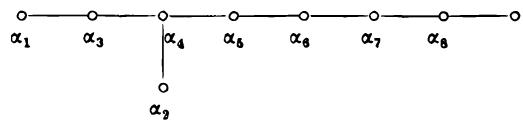
\includegraphics[keepaspectratio]{images/part002_295bff8e.jpg}}

\begin{enumerate}
\def\labelenumi{(\Alph{enumi})}
\setcounter{enumi}{21}
\tightlist
\item
  由于 \((\alpha |\alpha) = 2\) 对所有 \(\alpha \in \mathbb{R}\) 成立，所以 \(R^{\prime} = R\)。
\end{enumerate}

对于 \(\Phi_{\mathrm{R}}\)，根的长度平方为 \(\frac{1}{30}\)（ \(\S 1\)，第 12 号）。因此，\(\Phi_{\mathrm{R}}(x,y) = (x|y)/60\)，且 \(\gamma(\mathrm{R}) = 900\)（ \(\S 1\)，第 12 号，公式 (20)）。

\begin{enumerate}
\def\labelenumi{(\Roman{enumi})}
\setcounter{enumi}{5}
\tightlist
\item
  计算基本权得到
\end{enumerate}

\[
\begin{array}{l} \omega_ {1} = 2 \varepsilon_ {8} = 4 \alpha_ {1} + 5 \alpha_ {2} + 7 \alpha_ {3} + 10 \alpha_ {4} + 8 \alpha_ {5} + 6 \alpha_ {6} + 4 \alpha_ {7} + 2 \alpha_ {8} \\ \omega_ {2} = \frac {1}{2} (\varepsilon_ {1} + \varepsilon_ {2} + \varepsilon_ {3} + \varepsilon_ {4} + \varepsilon_ {5} + \varepsilon_ {6} + \varepsilon_ {7} + 5 \varepsilon_ {8}) \\ \qquad = 5 \alpha_ {1} + 8 \alpha_ {2} + 10 \alpha_ {3} + 15 \alpha_ {4} + 12 \alpha_ {5} + 9 \alpha_ {6} + 6 \alpha_ {7} + 3 \alpha_ {8} \\ \omega_ {3} = \frac {1}{2} (- \varepsilon_ {1} + \varepsilon_ {2} + \varepsilon_ {3} + \varepsilon_ {4} + \varepsilon_ {5} + \varepsilon_ {6} + \varepsilon_ {7} + 7 \varepsilon_ {8}) \\ \qquad = 7 \alpha_ {1} + 10 \alpha_ {2} + 14 \alpha_ {3} + 20 \alpha_ {4} + 16 \alpha_ {5} + 12 \alpha_ {6} + 8 \alpha_ {7} + 4 \alpha_ {8} \\ \omega_ {4} = \varepsilon_ {3} + \varepsilon_ {4} + \varepsilon_ {5} + \varepsilon_ {6} + \varepsilon_ {7} + 5 \varepsilon_ {8} \\ \qquad = 10 \alpha_ {1} + 15 \alpha_ {2} + 20 \alpha_ {3} + 30 \alpha_ {4} + 24 \alpha_ {5} + 18 \alpha_ {6} + 12 \alpha_ {7} + 6 \alpha_ {8} \\ \omega_ {5} = \varepsilon_ {4} + \varepsilon_ {5} + \varepsilon_ {6} + \varepsilon_ {7} + 4 \varepsilon_ {8} \\ \qquad = 8 \alpha_ {1} + 12 \alpha_ {2} + 16 \alpha_ {3} + 24 \alpha_ {4} + 20 \alpha_ {5} + 15 \alpha_ {6} + 10 \alpha_ {7} + 5 \alpha_ {8} \\ \omega_ {6} = \varepsilon_ {5} + \varepsilon_ {6} + \varepsilon_ {7} + 3 \varepsilon_ {8} \\ \qquad = 6 \alpha_ {1} + 9 \alpha_ {2} + 12 \alpha_ {3} + 18 \alpha_ {4} + 15 \alpha_ {5} + 12 \alpha_ {6} + 8 \alpha_ {7} + 4 \alpha_ {8} \\ \omega_ {7} = \varepsilon_ {6} + \varepsilon_ {7} + 2 \varepsilon_ {8} \\ \qquad = 4 \alpha_ {1} + 6 \alpha_ {2} + 8 \alpha_ {3} + 2 \alpha_ {4} + 10 \alpha_ {5} + 8 \alpha_ {6} + 6 \alpha_ {7} + 3 \alpha_ {8} \\ \omega_ {8} = \varepsilon_ {7} + \varepsilon_ {8} \\ \qquad = 5 \alpha_ {1} + 8 \alpha_ {2} + 10 \alpha_ {3} + 15 \alpha_ {4} + 12 \alpha_ {5} + 9 \alpha_ {6} + 6 \alpha_ {7} + 3 \alpha_ {8} = \tilde {\alpha}. \end{array}
\]

\begin{enumerate}
\def\labelenumi{(\Roman{enumi})}
\setcounter{enumi}{6}
\tightlist
\item
  正根之和的一半是基本权之和（§ 1，第 10 号，命题 29）；这给出
\end{enumerate}

\[
\begin{array}{r l} \rho & = \varepsilon_ {2} + 2 \varepsilon_ {3} + 3 \varepsilon_ {4} + 4 \varepsilon_ {5} + 5 \varepsilon_ {6} + 6 \varepsilon_ {7} + 23 \varepsilon_ {8} \\ & = 46 \alpha_ {1} + 68 \alpha_ {2} + 91 \alpha_ {3} + 135 \alpha_ {4} + 110 \alpha_ {5} + 84 \alpha_ {6} + 57 \alpha_ {7} + 29 \alpha_ {8}. \end{array}
\]

\begin{enumerate}
\def\labelenumi{(\Roman{enumi})}
\setcounter{enumi}{7}
\item
  群 \(Q(R)\) 由 \(\varepsilon_{i} \pm \varepsilon_{j}\) 和 \(\frac{1}{2} \sum_{i=1}^{8} \varepsilon_{i}\) 生成，并且等于 \(L_{3}\)（第 4 号）。因此，\(P(R)\)（与 \(Q(R^{\prime}) = Q(R) = L_{3}\) 关联）是 \(L_{3}\)（第 4 号）。连接指标为 1。
\item
  指数族有 8 项，由于 h = 30，与 30 互素的整数 1、7、11、13、17、19、23、29 必须出现在此族中；因此，这些就是 W(R) 的指数。
\item
  由 (IX) 以及第 V 章 § 6 第 2 号命题 3 的推论 1，得到 W(R) 的阶为
\end{enumerate}

\[
2. 8. 12. 14. 18. 20. 24. 30 = 2 ^ {14}. 3 ^ {5}. 5 ^ {2}. 7.
\]

\begin{enumerate}
\def\labelenumi{(\Roman{enumi})}
\setcounter{enumi}{10}
\tightlist
\item
  Dynkin 图的唯一自同构是恒等自同构，因为从分叉点发出的三条链长度各不相同。因此，\(A(R) = W(R)\) 且 \(w_{0} = -1\)。
\end{enumerate}

\subsection{\texorpdfstring{\(E_{7}\) 型系统}{E\_7 型系统}}

\begin{enumerate}
\def\labelenumi{(\Roman{enumi})}
\tightlist
\item
  以及 (II) 设 \(E = R^{8}\)，并令 \(R_{8}\) 为第 10 号在 E 中构造的根系。令 V 为 E 中由根 \(\alpha_{1}, \ldots, \alpha_{7}\)（它们属于 \(R_{8}\)）生成的超平面；它与第八个基本权 \(\omega = \varepsilon_{7} + \varepsilon_{8}\)（属于 \(R_{8}\)）正交。
\end{enumerate}

  令 \(R = R_{8} \cap V\)。则 \(R\) 是一个以 \((\alpha_{1}, \ldots, \alpha_{7})\) 为基的约化根系，参见 § 1，第 7 号，命题 20 的推论 4；因此，该系统为 \(E_{7}\) 型。其元素为：

\[
\begin{array}{c} \pm \varepsilon_ {i} \pm \varepsilon_ {j} (1 \leqslant i < j \leqslant 6), \quad \pm (\varepsilon_ {7} - \varepsilon_ {8}), \\ \pm \frac {1}{2} (\varepsilon_ {7} - \varepsilon_ {8} + \sum_ {i = 1} ^ {8} (- 1) ^ {\nu (i)} \varepsilon_ {i}) \quad \text { with } \sum_ {i = 1} ^ {8} \nu (i) \text { odd }. \end{array}
\]

根的数目为 \(n = 2 + \binom{6}{2}.4 + 2^6 = 126\)。正根为

\[
\pm \varepsilon_ {i} + \varepsilon_ {j} (1 \leqslant i <   j \leqslant 6). - \varepsilon_ {7} + \varepsilon_ {8},
\]

\[
\frac {1}{2} \left(- \varepsilon_ {7} + \varepsilon_ {8} + \sum_ {i = 1} ^ {6} (- 1) ^ {\nu (i)} \varepsilon_ {i}\right) \quad \text { with } \sum_ {i = 1} ^ {6} \nu (i) \text { odd }.
\]

\begin{enumerate}
\def\labelenumi{(\Roman{enumi})}
\setcounter{enumi}{2}
\item
  我们有 \(h = \frac{n}{l} = 18\)。
\item
  令 \(\tilde{\alpha} = \varepsilon_8 - \varepsilon_7 = 2\alpha_1 + 2\alpha_2 + 3\alpha_3 + 4\alpha_4 + 3\alpha_5 + 2\alpha_6 + \alpha_7\)，这是一个根。相对于 \((\alpha_i)\)，它的坐标之和为 \(17 = h - 1\)。因此它是最高根。它与 \(\alpha_i\)（\(2 \leqslant i \leqslant 7\)）正交，且 \((\tilde{\alpha}|\alpha_1) = 1\)。扩展 Dynkin 图为
\end{enumerate}

\pandocbounded{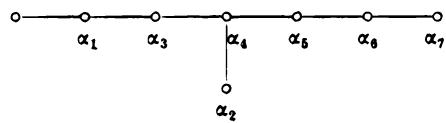
\includegraphics[keepaspectratio]{images/part002_8927380c.jpg}}

\begin{enumerate}
\def\labelenumi{(\Alph{enumi})}
\setcounter{enumi}{21}
\tightlist
\item
  由于 \((\alpha |\alpha) = 2\) 对所有 \(\alpha \in \mathbb{R}\) 成立，所以 \(R^{\prime} = R\)。
\end{enumerate}

对于 \(\Phi_{\mathrm{R}}\)，根的长度平方为 \(\frac{1}{18}\)，所以

\[
\Phi_ {\mathrm{R}} (x, y) = (x | y) / 36, \quad \text { and } \quad \gamma (\mathrm{R}) = 2 ^ {2}. 3 ^ {4}
\]

（§ 1，第 12 号，公式 (20)）。

\begin{enumerate}
\def\labelenumi{(\Roman{enumi})}
\setcounter{enumi}{5}
\tightlist
\item
  计算基本权得到
\end{enumerate}

\[
\begin{array}{r l} & {\omega_ {1} = \varepsilon_ {8} - \varepsilon_ {7} = 2 \alpha_ {1} + 2 \alpha_ {2} + 3 \alpha_ {3} + 4 \alpha_ {4} + 3 \alpha_ {5} + 2 \alpha_ {6} + \alpha_ {7}} \\ & {\omega_ {2} = \frac {1}{2} (\varepsilon_ {1} + \varepsilon_ {2} + \varepsilon_ {3} + \varepsilon_ {4} + \varepsilon_ {5} + \varepsilon_ {6} - 2 \varepsilon_ {7} + 2 \varepsilon_ {8})} \\ & {\qquad = \frac {1}{2} (4 \alpha_ {1} + 7 \alpha_ {2} + 8 \alpha_ {3} + 12 \alpha_ {4} + 9 \alpha_ {5} + 8 \alpha_ {6} + 3 \alpha_ {7})} \\ & {\omega_ {3} = \frac {1}{2} (- \varepsilon_ {1} + \varepsilon_ {2} + \varepsilon_ {3} + \varepsilon_ {4} + \varepsilon_ {5} + \varepsilon_ {6} - 3 \varepsilon_ {7} + 3 \varepsilon_ {8})} \\ & {\qquad = 3 \alpha_ {1} + 4 \alpha_ {2} + 6 \alpha_ {3} + 8 \alpha_ {4} + 6 \alpha_ {5} + 4 \alpha_ {6} + 2 \alpha_ {7}} \\ & {\omega_ {4} = \varepsilon_ {3} + \varepsilon_ {4} + \varepsilon_ {5} + \varepsilon_ {6} + 2 (\varepsilon_ {8} - \varepsilon_ {7})} \\ & {\qquad = 4 \alpha_ {1} + 6 \alpha_ {2} + 8 \alpha_ {3} + 12 \alpha_ {4} + 9 \alpha_ {5} + 6 \alpha_ {6} + 3 \alpha_ {7}} \\ & {\omega_ {5} = \varepsilon_ {4} + \varepsilon_ {5} + \varepsilon_ {6} + \frac {3}{2} (\varepsilon_ {8} - \varepsilon_ {7})} \\ & {\qquad = \frac {1}{2} (6 \alpha_ {1} + 9 \alpha_ {2} + 12 \alpha_ {3} + 18 \alpha_ {4} + 15 \alpha_ {5} + 10 \alpha_ {6} + 5 \alpha_ {7})} \\ & {\omega_ {6} = \varepsilon_ {5} + \varepsilon_ {6} - \varepsilon_ {7} + \varepsilon_ {8}} \\ & {\qquad = 2 \alpha_ {1} + 3 \alpha_ {2} + 4 \alpha_ {3} + 6 \alpha_ {4} + 5 \alpha_ {5} + 4 \alpha_ {6} + 2 \alpha_ {7}} \\ & {\omega_ {7} = \varepsilon_ {6} + \frac {1}{2} (\varepsilon_ {8} - \varepsilon_ {7})} \\ & {\qquad = \frac {1}{2} (2 \alpha_ {1} + 3 \alpha_ {2} + 4 \alpha_ {3} + 6 \alpha_ {4} + 5 \alpha_ {5} + 4 \alpha_ {6} + 3 \alpha_ {7}).} \end{array}
\]

\begin{enumerate}
\def\labelenumi{(\Roman{enumi})}
\setcounter{enumi}{6}
\tightlist
\item
  正根之和 \(2\rho\) 等于 \(2\sum_{i=1}^{7}\omega_i\)（§ 1，第 10 号，命题 29），所以
\end{enumerate}

\[
\begin{array}{r l} 2 \rho & = 2 \varepsilon_ {2} + 4 \varepsilon_ {3} + 6 \varepsilon_ {4} + 8 \varepsilon_ {5} + 10 \varepsilon_ {6} - 17 \varepsilon_ {7} + 17 \varepsilon_ {8} \\ & = 34 \alpha_ {1} + 49 \alpha_ {2} + 66 \alpha_ {3} + 96 \alpha_ {4} + 75 \alpha_ {5} + 52 \alpha_ {6} + 27 \alpha_ {7}. \end{array}
\]

\begin{enumerate}
\def\labelenumi{(\Roman{enumi})}
\setcounter{enumi}{7}
\tightlist
\item
  由第 10 号 (VIII) 及 § 1，第 10 号，命题 28，有
\end{enumerate}

\[
\mathrm{Q} (\mathrm{R}) = \mathrm{Q} (\mathrm{R} _ {8}) \cap \mathrm{V} = \mathrm{L} _ {3} \cap \mathrm{V} \quad \text { and } \quad \mathrm{P} (\mathrm{R}) = p (\mathrm{P} (\mathrm{R} _ {8})) = p (\mathrm{L} _ {3}),
\]

其中 p 表示 E 到 V 的正交投影。群 \(Q(R)\) 的基为 \((\alpha_{1},\ldots,\alpha_{7})\)；群 \(P(R)\) 由 \(Q(R)\) 和

\[
p (\alpha_ {8}) = \alpha_ {8} - \frac {1}{2} \omega .
\]

我们有 \(\omega\in\mathrm{P}(\mathrm{R}_{8})\)，\(\frac{1}{2}\omega\notin\mathrm{P}(\mathrm{R}_{8})\)，所以 \(2p(\alpha_{8})\in\mathrm{Q}(\mathrm{R})\) 而 \(p(\alpha_{8})\notin\mathrm{Q}(\mathrm{R})\)。因此，\(\mathrm{P}(\mathrm{R})/\mathrm{Q}(\mathrm{R})\) 同构于 Z/2Z，并由例如 \(\omega_{7}\) 的像生成。

连接指标为 2。

\begin{enumerate}
\def\labelenumi{(\Roman{enumi})}
\setcounter{enumi}{8}
\tightlist
\item
  \(W(R)\) 的指数序列有 7 项。与 \(h = 18\) 互素的数 1、5、7、11、13、17 出现在此序列中。最后一个指数 \(m\) 必须满足 \(m + m = 18\)（第 V 章，§ 6，第 2 号，公式 (2)）。因此，指数序列为
\end{enumerate}

\[
1, 5, 7, 9, 11, 13, 17.
\]

\begin{enumerate}
\def\labelenumi{(\Alph{enumi})}
\setcounter{enumi}{23}
\tightlist
\item
  由 (IX) 及第 V 章 § 6 第 2 号命题 3 的推论 1，得到 W(R) 的阶为
\end{enumerate}

\[
2. 6. 8. 10. 12. 14. 18 = 2 ^ {10}. 3 ^ {4}. 5. 7.
\]

\begin{enumerate}
\def\labelenumi{(\Roman{enumi})}
\setcounter{enumi}{10}
\item
  Dynkin 图的唯一自同构是恒等自同构，所以 \(\mathbf{A}(\mathbf{R}) = \mathbf{W}(\mathbf{R})\) 且 \(w_0 = -1\)。
\item
  \(\mathrm{P}(\mathrm{R}^{-})/\mathrm{Q}(\mathrm{R}^{-})\) 只有一个非单位元。它互换对应于 \(\alpha_{0}\) 和 \(\alpha_{7}\)、\(\alpha_{1}\) 和 \(\alpha_{6}\)、\(\alpha_{3}\) 和 \(\alpha_{5}\) 的顶点，并固定 \(\alpha_{2}\) 和 \(\alpha_{4}\)。
\end{enumerate}

\subsection{\texorpdfstring{\(E_{6}\) 型系统}{E\_6 型系统}}

\begin{enumerate}
\def\labelenumi{(\Roman{enumi})}
\tightlist
\item
  以及 (II) 设 \(E = R^{8}\) ，并令 \(R_{8}\) 为第 10 号中构造的 E 中的根系。令 V 为 E 中由根 \(\alpha_{1}, \ldots, \alpha_{6}\)（属于 \(R_{8}\)）所生成的向量子空间；它是由最后两个基本权 \(\omega = \varepsilon_{7} + \varepsilon_{8}\) 和 \(\pi = \varepsilon_{6} + \varepsilon_{7} + 2\varepsilon_{8}\)（属于 \(R_{8}\)）所生成平面的正交补。
\end{enumerate}

令 \(R = R_{8} \cap V\) 。这是一个以 \((\alpha_{1}, \ldots, \alpha_{6})\) 为基的约化根系，因而是 \(E_{6}\) 型的根系。其元素为：

\[
\begin{array}{c} \pm \varepsilon_ {i} \pm \varepsilon_ {j} (1 \leqslant i <   j \leqslant 5), \\ \pm \frac {1}{2} (\varepsilon_ {8} - \varepsilon_ {7} - \varepsilon_ {6} + \sum_ {i = 1} ^ {5} (- 1) ^ {\nu (i)} \varepsilon_ {i}) \text {with} \sum_ {i = 1} ^ {5} \nu (i) \text {even.} \end{array}
\]

根的数目为 \(n = \binom{5}{2}.4 + 2^5 = 72\) 。正根为

\[
\pm \varepsilon_ {i} + \varepsilon_ {j} (1 \leqslant i <   j \leqslant 5),
\]

\[
\frac {1}{2} \left(\varepsilon_ {8} - \varepsilon_ {7} - \varepsilon_ {6} + \sum_ {i = 1} ^ {5} (- 1) ^ {\nu (i)} \varepsilon_ {i}\right) \text {with} \sum_ {i = 1} ^ {5} \nu (i) \text {even}.
\]

\begin{enumerate}
\def\labelenumi{(\Roman{enumi})}
\setcounter{enumi}{2}
\item
  我们有 \(h = \frac{n}{6} = 12\) 。
\item
  令
\end{enumerate}

\[
\begin{array}{r l} \tilde {\alpha} & = \frac {1}{2} (\varepsilon_ {1} + \varepsilon_ {2} + \varepsilon_ {3} + \varepsilon_ {4} + \varepsilon_ {5} - \varepsilon_ {6} - \varepsilon_ {7} + \varepsilon_ {8}) \\ & = \alpha_ {1} + 2 \alpha_ {2} + 2 \alpha_ {3} + 3 \alpha_ {4} + 2 \alpha_ {5} + \alpha_ {6}, \end{array}
\]

这是一个根。相对于 \((\alpha_{i})\) ，其坐标之和为 11 = h - 1，因此 \(\tilde{\alpha}\) 是最高根。它与 \(\alpha_{1}, \alpha_{3}, \alpha_{4}, \alpha_{5}, \alpha_{6}\) 正交，且 \((\tilde{\alpha}|\alpha_{2}) = 1\) 。扩充的 Dynkin 图为

\pandocbounded{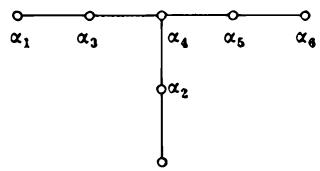
\includegraphics[keepaspectratio]{images/part002_9f0044a9.jpg}}

\begin{enumerate}
\def\labelenumi{(\Alph{enumi})}
\setcounter{enumi}{21}
\tightlist
\item
  由于 \((\alpha |\alpha) = 2\) 对所有 \(\alpha \in \mathbb{R}\) 成立，所以 \(\mathbb{R}^{\sim} = \mathbb{R}\) 。对于 \(\Phi_{\mathbb{R}}\) ，根的长度平方为 \(\frac{1}{12}\) ，因此
\end{enumerate}

\[
\Phi_ {\mathrm{R}} (x, y) = (x | y) / 24, \quad \text { and } \quad \gamma (\mathrm{R}) = 144.
\]

\begin{enumerate}
\def\labelenumi{(\Roman{enumi})}
\setcounter{enumi}{5}
\tightlist
\item
  计算基本权得到：
\end{enumerate}

\[
\begin{array}{l} \omega_ {1} = \frac {2}{3} (\varepsilon_ {8} - \varepsilon_ {7} - \varepsilon_ {6}) = \frac {1}{3} (4 \alpha_ {1} + 3 \alpha_ {2} + 5 \alpha_ {3} + 6 \alpha_ {4} + 4 \alpha_ {5} + 2 \alpha_ {6}) \\ \omega_ {2} = \frac {1}{2} (\varepsilon_ {1} + \varepsilon_ {2} + \varepsilon_ {3} + \varepsilon_ {4} + \varepsilon_ {5} - \varepsilon_ {6} - \varepsilon_ {7} + \varepsilon_ {8}) \\ \quad = \alpha_ {1} + 2 \alpha_ {2} + 2 \alpha_ {3} + 3 \alpha_ {4} + 2 \alpha_ {5} + \alpha_ {6} = \tilde {\alpha} \\ \omega_ {3} = \frac {5}{6} (\varepsilon_ {8} - \varepsilon_ {7} - \varepsilon_ {6}) + \frac {1}{2} (- \varepsilon_ {1} + \varepsilon_ {2} + \varepsilon_ {3} + \varepsilon_ {4} + \varepsilon_ {5}) \\ \quad = \frac {1}{3} (5 \alpha_ {1} + 6 \alpha_ {2} + 10 \alpha_ {3} + 12 \alpha_ {4} + 8 \alpha_ {5} + 4 \alpha_ {6}) \\ \omega_ {4} = \varepsilon_ {3} + \varepsilon_ {4} + \varepsilon_ {5} - \varepsilon_ {6} - \varepsilon_ {7} + \varepsilon_ {8} \\ \quad = 2 \alpha_ {1} + 3 \alpha_ {2} + 4 \alpha_ {3} + 6 \alpha_ {4} + 4 \alpha_ {5} + 2 \alpha_ {6} \\ \omega_ {5} = \frac {2}{3} (\varepsilon_ {8} - \varepsilon_ {7} - \varepsilon_ {6}) + \varepsilon_ {4} + \varepsilon_ {5} \\ \quad = \frac {1}{3} (4 \alpha_ {1} + 6 \alpha_ {2} + 8 \alpha_ {3} + 12 \alpha_ {4} + 10 \alpha_ {5} + 5 \alpha_ {6}) \\ \omega_ {6} = \frac {1}{3} (\varepsilon_ {8} - \varepsilon_ {7} - \varepsilon_ {6}) + \varepsilon_ {5} \\ \quad = \frac {1}{3} (2 \alpha_ {1} + 3 \alpha_ {2} + 4 \alpha_ {3} + 6 \alpha_ {4} + 5 \alpha_ {5} + 4 \alpha_ {6}). \end{array}
\]

\begin{enumerate}
\def\labelenumi{(\Roman{enumi})}
\setcounter{enumi}{6}
\tightlist
\item
  正根之和的一半是 \(\sum_{i=1}^{6} \omega_i\) ，所以
\end{enumerate}

\[
\begin{array}{r l} \rho & = \varepsilon_ {2} + 2 \varepsilon_ {3} + 3 \varepsilon_ {4} + 4 \varepsilon_ {5} + 4 (\varepsilon_ {8} - \varepsilon_ {7} - \varepsilon_ {6}) \\ & = 8 \alpha_ {1} + 11 \alpha_ {2} + 15 \alpha_ {3} + 21 \alpha_ {4} + 15 \alpha_ {5} + 8 \alpha_ {6}. \end{array}
\]

\begin{enumerate}
\def\labelenumi{(\Roman{enumi})}
\setcounter{enumi}{7}
\tightlist
\item
  由第 10 号 (VIII) 及 § 1，第 10 号，命题 28，
\end{enumerate}

\[
\mathrm{Q} (\mathrm{R}) = \mathrm{Q} (\mathrm{R} _ {8}) \cap \mathrm{V} = \mathrm{L} _ {3} \cap \mathrm{V} \quad \text { and } \quad \mathrm{P} (\mathrm{R}) = p (\mathrm{P} (\mathrm{R} _ {8})) = p (\mathrm{L} _ {3}),
\]

其中 p 表示从 E 到 V 的正交投影。我们有

\[
p (\alpha_ {7}) = \alpha_ {7} - \frac {2}{3} \pi + \omega , \quad p (\alpha_ {8}) = \alpha_ {8} + \pi - 2 \omega .
\]

群 \(Q(R)\) 的基为 \((\alpha_{1},\ldots,\alpha_{6})\) 。群 \(P(R)\) 由 \(Q(R)\) 和 \(p(\alpha_{7})\) 生成，因为 \(p(\alpha_{8})\in P(R_{8})\cap V=Q(R_{8})\cap V=Q(R)\) 。我们有 \(3p(\alpha_{7})\in Q(R)\) 且 \(p(\alpha_{7})\notin Q(R)\) 。因此，群 \(P(R)/Q(R)\) 同构于 Z/3Z；例如，它由 \(\omega_{6}\) 的像生成。

连通指标为 3。

\begin{enumerate}
\def\labelenumi{(\Roman{enumi})}
\setcounter{enumi}{8}
\tightlist
\item
  (IX) 和 (X) 由 § 2，第 4 号，命题 7，Weyl 群的阶为 6!1.2.2.3.2.1.3 = \(2^{7}.3^{4}.5\) 。指数序列在 1 与 11 之间有 6 项，并包含与 12 互素的整数 1、5、7、11。其他指数 \(m, m'\) 是满足
\end{enumerate}

\[
m + m ^ {\prime} = 12.
\]

\[
(m + 1) \left(m ^ {\prime} + 1\right) (1 + 1) (5 + 1) (7 + 1) (11 + 1) = 2 ^ {7}. 3 ^ {4}. 5,
\]

根据第 V 章 § 6，第 2 号，公式 (2) 以及命题 3 的推论 1。第二个关系给出 \((m + 1)(m' + 1) = 45\) ，又因 \(m + m' + 2 = 14\) ，得到 \(m = 4\) ，\(m' = 8\) 。因此，指数序列为

\[
1, 4, 5, 7, 8, 11.
\]

\begin{enumerate}
\def\labelenumi{(\Roman{enumi})}
\setcounter{enumi}{10}
\tightlist
\item
  (XI) 和 (XII) 由于所有根的长度都相同，Dynkin 图的自同构就是底层图的自同构。除恒等自同构外，只有自同构 \(\varepsilon\) 将 \(\alpha_{1},\alpha_{3},\alpha_{4},\alpha_{5},\alpha_{6},\) \(\alpha_{2}\) 分别变为 \(\alpha_{6},\alpha_{5},\alpha_{4},\alpha_{3},\alpha_{1},\alpha_{2}\) 。因此，\(\mathrm{A(R) / W(R)}\) 同构于 \(\mathbf{Z} / 2\mathbf{Z}\) ；由于 \(-1\in \mathrm{W(R)}\) （第 V 章 §6，第 2 号，命题 3 的推论 3），\(\mathrm{A(R)}\) 同构于 \(\mathrm{W(R)}\times \{1, - 1\}\) ，且可将 \(w_0\) 认作 \(-\varepsilon\) 。由此，\(\mathrm{A(R) / W(R)}\) 的非恒等元素定义了自同构 \(x\mapsto -x\)，该自同构作用于 \(\mathrm{P(R^{\prime}) / Q(R^{\prime})}\)。
\end{enumerate}

此外，\(P(R^{-})/Q(R^{-})\) 有两个阶为 3 的非恒等元素。它们定义了扩充 Dynkin 图的两个三阶自同构。

\subsection{\texorpdfstring{\(G_{2}\) 型系统}{G\_2 型系统}}

\begin{enumerate}
\def\labelenumi{(\Roman{enumi})}
\tightlist
\item
  令 E 为 \(R^{3}\) 中方程为
\end{enumerate}

\[
\xi_ {1} + \xi_ {2} + \xi_ {3} = 0.
\]

  令 \(R\) 为由 \(\alpha \in L_0 \cap V\) 且满足 \((\alpha | \alpha) = 2\) 或 \((\alpha | \alpha) = 6\) 的元素组成的集合。\(R\) 的元素为

\[
\begin{array}{c} \pm (\varepsilon_ {1} - \varepsilon_ {2}), \quad \pm (\varepsilon_ {1} - \varepsilon_ {3}), \quad \pm (\varepsilon_ {2} - \varepsilon_ {3}), \quad \pm (2 \varepsilon_ {1} - \varepsilon_ {2} - \varepsilon_ {3}), \\ \pm (2 \varepsilon_ {2} - \varepsilon_ {1} - \varepsilon_ {3}), \quad \pm (2 \varepsilon_ {3} - \varepsilon_ {1} - \varepsilon_ {2}). \end{array}
\]

  于是，R 生成 V，且 \(\frac{2(\alpha|\beta)}{(\beta|\beta)}\in\mathbf{Z}\) 对所有 \(\alpha,\beta\in R\) 成立：当 \(\beta=\pm(\varepsilon_{i}-\varepsilon_{j})\) 且 \(i\neq j\) 时这显然成立；例如，当 \(\beta=2\varepsilon_{1}-\varepsilon_{2}-\varepsilon_{3}\) 时，我们有 \((\alpha|\beta)\in3\mathbf{Z}\) ，断言同样成立。因此，R 是 V 中的约化根系。根的数目为 n=12。

\begin{enumerate}
\def\labelenumi{(\Roman{enumi})}
\setcounter{enumi}{1}
\tightlist
\item
  置 \(\alpha_{1} = \varepsilon_{1} - \varepsilon_{2},\alpha_{2} = -2\varepsilon_{1} + \varepsilon_{2} + \varepsilon_{3}\) 。则这些根为
\end{enumerate}

\[
\begin{array}{r l} & {\pm \alpha_ {1}, \quad \pm (\alpha_ {1} + \alpha_ {2}), \quad \pm (2 \alpha_ {1} + \alpha_ {2}), \quad \pm \alpha_ {2},} \\ & {\qquad \pm (3 \alpha_ {1} + \alpha_ {2}), \quad \pm (3 \alpha_ {1} + 2 \alpha_ {2}).} \end{array}
\]

因此，\((\alpha_{1},\alpha_{2})\) 是 \(R\) 的一个基。我们有 \(\| \alpha_{1}\|^{2} = 2,\| \alpha_{2}\|^{2} = 6.\) \((\alpha_{1}|\alpha_{2}) = -3,\) 所以 \(R\) 是 \(G_{2}\) 型系统。正根为 \(\alpha_{1},\alpha_{1} + \alpha_{2},2\alpha_{1} + \alpha_{2},\) \(3\alpha_{1} + \alpha_{2},3\alpha_{1} + 2\alpha_{2}\) 。

\begin{enumerate}
\def\labelenumi{(\Roman{enumi})}
\setcounter{enumi}{2}
\item
  我们有 \(h = \frac{n}{2} = 6\) 。
\item
  最高根为 \(\tilde{\alpha} = 3\alpha_{1} + 2\alpha_{2} = -\varepsilon_{1} - \varepsilon_{2} + 2\varepsilon_{3}\) 。我们有 \((\tilde{\alpha}|\alpha_{1}) = 0, (\tilde{\alpha}|\alpha_{2}) = 3\) 。扩充的 Dynkin 图为
\end{enumerate}

\[
\alpha_ {1} \quad \alpha_ {2}
\]

\begin{enumerate}
\def\labelenumi{(\Alph{enumi})}
\setcounter{enumi}{21}
\tightlist
\item
  逆系统是下列向量集：
\end{enumerate}

\[
\begin{array}{l} \pm \alpha_ {1}, \quad \pm (\alpha_ {1} + \alpha_ {2}), \quad \pm (2 \alpha_ {1} + \alpha_ {2}), \quad \pm \frac {1}{3} \alpha_ {2}, \\ \qquad \pm \frac {1}{3} (3 \alpha_ {1} + \alpha_ {2}), \quad \pm \frac {1}{3} (3 \alpha_ {1} + 2 \alpha_ {2}). \end{array}
\]

  有 10 个根不与 \(\alpha_{1}\) 正交；其中 4 个根满足 \(n(\beta, \alpha_{1}) = \pm 1\) ，另外 4 个满足 \(n(\beta, \alpha_{1}) = \pm 3\) ，另有 \(n(\beta, \alpha_{1}) = \pm 2\) 的根满足 \(\beta = \pm \alpha_{1}\) 。因此，\(\alpha_{1}\) 在 \(\Phi_{\mathbb{R}}\) 中的长度平方为 \(4(4.1 + 4.9 + 2.4)^{-1} = \frac{1}{12}\) 。从而 \(\Phi_{\mathbb{R}}(x, y) = (x|y)/24\) 。现在对 \(x = y = \alpha_{1}\) 应用 §1 第 12 号的公式 (18)，得到

\[
2 + 4. \frac {1}{4} + 4. \frac {1}{4} = \gamma (\mathrm{R}). \frac {1}{12}
\]

所以 \(\gamma (\mathbb{R}) = 48\)

\begin{enumerate}
\def\labelenumi{(\Roman{enumi})}
\setcounter{enumi}{5}
\tightlist
\item
  (VI) 和 (VII) 正根之和的一半为
\end{enumerate}

\[
\rho = 5 \alpha_ {1} + 3 \alpha_ {2}.
\]

基本权 \(\omega_{1}\) 和 \(\omega_{2}\) 分别与 \(\alpha_{2}\) 和 \(\alpha_{1}\) 正交，因而分别与 \(2\alpha_{1} + \alpha_{2}\) 和 \(3\alpha_{1} + 2\alpha_{2}\) 成比例。我们有

\[
\omega_ {1} + \omega_ {2} = \rho = 5 \alpha_ {1} + 3 \alpha_ {2} = (2 \alpha_ {1} + \alpha_ {2}) + (3 \alpha_ {1} + 2 \alpha_ {2}).
\]

因此，

\[
\omega_ {1} = 2 \alpha_ {1} + \alpha_ {2}, \quad \omega_ {2} = 3 \alpha_ {1} + 2 \alpha_ {2} = \tilde {\alpha}.
\]

\begin{enumerate}
\def\labelenumi{(\Roman{enumi})}
\setcounter{enumi}{7}
\item
  例如，Q(R) 由 \(\varepsilon_{1}-\varepsilon_{2}\) 和 \(\varepsilon_{1}-\varepsilon_{3}\) 生成。由 (VI) 和 (VII)，P(R) = Q(R)。连通指标为 1。
\item
  指数族有 2 项：由于 1 和 \(h - 1 = 5\) 是指数，它们就是全部指数。
\item
  我们有 \((\alpha_{1},\alpha_{2}) = \frac{5\pi}{6}\) ，所以 \(\mathrm{W}(\mathbb{R})\) 同构于阶为 12 的二面体群。
\item
  Dynkin 图的唯一自同构是恒等自同构，所以 \(A(R) = W(R)\) 且 \(w_{0} = -1\) 。
\end{enumerate}

\subsection{不可约非约化根系}

利用 §1 第 4 号的命题 13 和 14，可以从不可约约化根系得到不可约非约化根系。对每个整数 \(l \geqslant 1\) ，存在一个秩为 \(l\) 的不可约非约化根系，且在同构意义下唯一：令 \(R\) 为 \(B_l\) 型根系。令 A 为 \(R\) 的最短根的集合；取 \(R\) 与 \(2A\) 的并。采用第 5 号的记号，我们得到 \(2l(l + 1)\) 个向量

\[
\pm \varepsilon_ {i}, \quad \pm 2 \varepsilon_ {i}, \quad \varepsilon_ {i} \pm \varepsilon_ {j} (i <   j).
\]

\exercisesection{§ 1 的习题}

下文考虑的所有根系都相对于实向量空间。我们用 \((x|y)\) 表示在 Weyl 群下不变的标量积（参见第 3 号）。

\begin{enumerate}
\def\labelenumi{\arabic{enumi})}
\item
  令 \(\mathbb{R}\) 为根系，\(\mathbb{R} = \mathbb{R}_1 \cup \mathbb{R}_2\) 为 \(\mathbb{R}\) 的一个划分。假设，当 \(x, y\) 是 \(\mathbb{R}_i\) 的两个元素且 \(x + y\)（分别为 \(x - y\)）是一个根时，就有 \(x + y \in \mathbb{R}_i\)（分别为 \(x - y \in \mathbb{R}_i\)），其中 \(i = 1, 2\)。那么，\(\mathbb{R}\) 是 \(\mathbb{R}_1\) 与 \(\mathbb{R}_2\) 的直和。（利用第 3 号定理 1 的推论，证明若 \(x \in \mathbb{R}_1\) 且 \(y \in \mathbb{R}_2\)，则 \((x|y) = 0\)。）
\item
  令 R 为根系，\(\alpha\) 和 \(\beta\) 为两个根。若 t 是一个标量且 \(\beta + t\alpha \in R\) ，则 \(2t \in Z\) 。（因为 \(n(\beta + t\alpha, \alpha) = n(\beta, \alpha) + 2t\) 。）若 \(\alpha\) 不可整除，则 \(t \in Z\) 。（否则利用命题 9 证明存在一个根 \(\gamma\)，它与 \(\alpha\) 正交，使得 \(\gamma + \frac{1}{2}\alpha \in R\)：于是 \((\gamma + \frac{1}{2}\alpha|\alpha) > 0\) ，所以 \(\frac{1}{2}\alpha \in R\)。）
\item
  令 R 为 V 中的不可约非约化根系。V 上存在一个非退化对称双线性型 \(\Phi\)，使得当将 V 与 \(V^{*}\) 通过 \(\Phi\) 识别时，有 \(R = R^{-}\)。（利用命题 13。）
\item
  令 \(\Gamma\) 为有限秩自由 \(\mathbf{Z}\)-模，其秩为 \(l\)，\(\Gamma^{*}\) 为其对偶 \(\mathbf{Z}\)-模，I 为有限指标集，\((x_{i}, x_{i}^{*})_{i \in \mathbf{I}}\) 为 \(\Gamma \times \Gamma^{*}\) 中的元素族，且满足 \(\langle x_{i}, x_{i}^{*} \rangle = 2\) 对所有 \(i \in \mathbf{I}\) 成立，\(s_{i} = s_{x_{i}, x_{i}^{*}}\)。令 \(\mathbf{V}\) 为实向量空间 \(\Gamma \otimes_{\mathbf{Z}} \mathbf{R}\)，其对偶 \(\mathbf{V}^{*}\) 可与 \(\Gamma^{*} \otimes_{\mathbf{Z}} \mathbf{R}\) 识别。我们也用 \(s_{i}\) 表示反射 \(s_{i} \otimes 1\) 在 \(\mathbf{V}\) 中的作用。令 \(\mathbf{R}\)（分别为 \(\mathbf{R}'\)）为 \(x_{i}\)（分别为 \(x_{i}^{*}\)）的集合。令 \(\mathbf{E}\)（分别为 \(\mathbf{E}'\)）为 \(\mathbf{V}\)（分别为 \(\mathbf{V}^{*}\)）中由 \(\mathbf{R}\)（分别为 \(\mathbf{R}'\)）生成的子空间。假设 \(s_{i}(\mathbf{R}) = \mathbf{R}\) 对所有 \(i\) 成立。那么，\(\mathbf{R}\) 是 \(\mathbf{E}\) 中的根系。\(\mathbf{E}'\) 可自然地识别为 \(\mathbf{E}\) 的对偶，且 \(x_{i}^{*}\) 可与 \(x_{i}^{-}\) 识别，对所有 \(i\) 均如此。若 \(\mathbf{F}\)（分别为 \(\mathbf{F}'\)）是 \(\mathbf{V}\)（分别为 \(\mathbf{V}^{*}\)）中在所有 \(s_{i}\)（分别为 \(^t s_{i}\)）下不变的点所成的子空间，则 \(\Gamma \cap \mathbf{F}\)（分别为 \(\Gamma^{*} \cap \mathbf{F}'\)）生成 \(\mathbf{F}\)（分别为 \(\mathbf{F}'\)）。若置 \(\Gamma_{1} = (\Gamma \cap \mathbf{E}) \oplus (\Gamma \cap \mathbf{F})\)（分别为 \(\Gamma_{1}^{*} = (\Gamma^{*} \cap \mathbf{E}') \oplus (\Gamma^{*} \cap \mathbf{F}')\)），则 \(\Gamma / \Gamma_{1}\) 与 \(\Gamma^{*} / \Gamma_{1}^{*}\) 是同构的有限群。
\item
  令 \(R\) 为不可约根系。对任意 \(\beta \in R\)，
\end{enumerate}

\[
16 \gamma (\mathrm{R}) = (\sum_ {\alpha \in \mathrm{R}} n (\alpha , \beta) ^ {2}) (\sum_ {\alpha \in \mathrm{R}} n (\beta , \alpha) ^ {2})
\]

从而 \(\gamma (\mathbb{R}) = \gamma (\lambda R)\) 对任意非零标量 \(\lambda\) 成立。（利用第 12 号的公式 (17) 和 (19)。）

\begin{enumerate}
\def\labelenumi{\arabic{enumi})}
\setcounter{enumi}{5}
\tightlist
\item
  \begin{enumerate}
  \def\labelenumii{\alph{enumii})}
  \tightlist
  \item
    令 A 为有限型阿贝尔群，T 为 A 的一个不含 0 的有限子集。存在 A 的有限指数子群 H，使得 \(H \cap T = \varnothing\)。（令 \(t \in T\)。利用有限型阿贝尔群的结构，构造 A 的一个不含 t 的有限指数子群。然后对 \(\text{Card}(T)\) 作归纳。）
  \end{enumerate}
\end{enumerate}

\begin{enumerate}
\def\labelenumi{\alph{enumi})}
\setcounter{enumi}{1}
\tightlist
\item
  令 R 为根系，P 为 R 的一个闭对称子集。存在 Q(R) 的有限指数子群 H，使得 \(P = H \cap R\)。（对 Q(R) 中由 P 生成的子群取商，并利用 a) 和命题 23。）
\end{enumerate}

\begin{enumerate}
\def\labelenumi{\arabic{enumi})}
\setcounter{enumi}{6}
\item
  根系的连通指标等于其 Cartan 矩阵的行列式。（利用第 10 号的公式 (14)。另一方面证明：在带有标量积的实向量空间中，若 \((\varepsilon_1, \ldots, \varepsilon_n), (\varepsilon_1', \ldots, \varepsilon_n')\) 是满足 \((\varepsilon_i | \varepsilon_j') = \delta_{ij}\) 的两个基，则 \(\det_{(\varepsilon_1, \ldots, \varepsilon_n)} (\varepsilon_1', \ldots, \varepsilon_n') > 0\)。）
\item
  令 R 为约化根系，C 为一个室，\(2\sigma\) 为 \(R^{-}\) 的正元素之和，\(P'(R)\) 为满足 \(x \in P(R)\) 且 \(\langle x, \sigma \rangle \in Z\) 的集合。于是，\(Q(R) \subseteq P'(R) \subseteq P(R)\)，且 \(P(R)/P'(R)\) 的阶为 1 或 2。令 \((\beta_{1}, \ldots, \beta_{l})\) 为与 C 对应的 \(R^{-}\) 的基，并置 \(2\sigma = n_{1}\beta_{1} + \cdots + n_{l}\beta_{l}\)，其中 \(n_{i}\) 是 \textgreater0 的整数。则 \(P(R) = P'(R)\) 当且仅当所有 \(n_{i}\) 都是偶数。
\item
  令 \(\mathbb{R}\) 为根系，\(\mathbb{C}\) 为一个室。置 \(\mathrm{B}(\mathbb{C}) = \{\alpha_1, \ldots, \alpha_l\}\)，
\end{enumerate}

\[
\mathrm{R} _ {+} (\mathrm{C}) = \left\{\alpha_ {1}, \dots , \alpha_ {l}, \alpha_ {l + 1}, \dots , \alpha_ {s} \right\}
\]

（其中 \(\alpha_{i}\) 两两不同），并令 \(\alpha = \alpha_{1} + \dots +\alpha_{s}\)。

\begin{enumerate}
\def\labelenumi{\alph{enumi})}
\tightlist
\item
  对 \(i = 1, 2, \ldots, s\) ，置 \(\varepsilon_{i} = \pm 1\)。令 \(\alpha^{*} = \varepsilon_{1}\alpha_{1} + \cdots + \varepsilon_{s}\alpha_{s}\)。若 \((\alpha^{*}|\alpha_{i}) > 0\) 对 \(i = 1, \ldots, l\) 成立，则 \(\alpha^{*} = \alpha\) 且对所有 i 都有 \(\varepsilon_{i} = 1\)。（令 \(\gamma\)（分别为 \(\delta\)）为 \(\alpha_{i}\) 之和，其中 \(\varepsilon_{i} = 1\)（分别为 -1）。则 \((\gamma|\alpha_{i}) - (\delta|\alpha_{i}) > 0\)，\((\gamma|\alpha_{i}) + (\delta|\alpha_{i}) = (\alpha_{i}|\alpha_{i})\)，所以
\end{enumerate}

\(2(\gamma|\alpha_{i})>(\alpha_{i}|\alpha_{i});\) 由于 \(2(\gamma|\alpha_{i}) / (\alpha_{i}|\alpha_{i})\in \mathbf{Z},(\gamma |\alpha_{i})\geqslant (\alpha_{i}|\alpha_{i}) = (\alpha |\alpha_{i}),\) 因而 \(\gamma -\alpha \in \overline{\mathrm{C}}. \gamma \geqslant \alpha ,\) \(\gamma = \alpha\) 且 \(\delta = 0.)\)

\begin{enumerate}
\def\labelenumi{\alph{enumi})}
\setcounter{enumi}{1}
\tightlist
\item
  对 \(i = 1,2,\ldots,s\)，令 \(\varepsilon_{i} = \pm 1\)。\(\varepsilon_{i}\alpha_{i}\)（\(>0\)）所成的集合是相对于某个室的正根集合，当且仅当 \(\alpha^{*} = \sum_{i}\varepsilon_{i}\alpha_{i}\) 属于某个室。（为证明充分性，令 \(\mu_{i} = \pm 1\) 满足 \((\alpha^{*}|\mu_{i}\alpha_{i}) > 0\)。存在 \(w\in W(R)\)，将 \(\mu_{i}\alpha_{i}\) 的集合变为 \(\alpha_{i}\) 的集合，从而将 \(\alpha^{*}\) 变为 \(\alpha^{**} = \sum_{i}\varepsilon_{i}\mu_{i}\alpha_{\sigma(i)}\)，其中 \(\sigma \in \mathfrak{S}_s\)。应用 \(a\)，证明 \(\alpha^{**} = \alpha\)，所以 \(\mu_{i}\varepsilon_{i} = 1\)。)
\end{enumerate}

\begin{enumerate}
\def\labelenumi{\arabic{enumi})}
\setcounter{enumi}{9}
\item
  令 \(\alpha\) 为不可约约化根系 R 相对于某个基的最高根。当且仅当所有根长度相同时，\(\alpha^{-}\) 才是 \(R^{-}\) 的最高根。
\item
  采用第 11 号命题 33 的记号，证明 \(\theta_{i} + \theta_{j}\) 对任意一对 \((i,j)\) 都不是根。
\item
  令 R 为 V 中秩 \(\geqslant 3\) 的根系，\((\alpha_{1},\ldots,\alpha_{l})\) 为 R 的一个基。令 \(V'\)（分别为 \(V''\)）为 V 中由 \(\alpha_{i}\) 生成的子空间，其中 \(i \geqslant 2\)（分别为 \(i \geqslant 3\)）。令 \(R' = R \cap V'\)，\(R'' = R \cap V''\)。令 d（分别为 \(d', d''\)）为 R（分别为 \(R', R''\)）的 Cartan 矩阵的行列式。假设 \(\alpha_{1}\) 与所有 \(\alpha_{i}\)（除 \(\alpha_{2}\) 外）正交，且 \(\| \alpha_{1} \| = \| \alpha_{2} \|\)。证明 \(d = 2d' - d''\)。
\item
  令 R 为约化根系。\((\alpha_{1},\ldots,\alpha_{l})\) 为 R 的一个基，且 \(\alpha=c_{1}\alpha_{1}+\cdots+c_{l}\alpha_{l}\) 为一个根。则对所有 i 都有 \(c_{i}(\alpha_{i}|\alpha_{i})/(\alpha|\alpha)\in\mathbf{Z}\)。（考虑逆系统。）
\item
  令 R 为不可约根系，\(\lambda\) 为最大的根长。令 S 为由长度为 \(\lambda\) 且两两正交的根组成的 R 的子集所成的集合。则 S 的任意两个极大元素都可由 W(R) 的元素彼此变换。（利用第 V 章 §3 第 3 号的命题 11 和命题 1。）
\item
  令 \(R\) 为秩为 \(l\) 的根系。
\end{enumerate}

\begin{enumerate}
\def\labelenumi{\alph{enumi})}
\item
  当且仅当 R 含有 l 个两两强正交的根时，\(-1 \in \mathrm{W}(\mathrm{R})\)。（为证明必要性，利用第 V 章 §3 第 3 号的命题 1 对 l 作归纳。）
\item
  若 \(w \in \mathrm{W}(\mathrm{R})\) 的阶为 2，则存在一个由两两强正交的根组成的集合 S，使得 w 是 \(s_{\alpha} (\alpha \in \mathrm{S})\) 的乘积。
\end{enumerate}

\begin{enumerate}
\def\labelenumi{\arabic{enumi})}
\setcounter{enumi}{15}
\tightlist
\item
  令 \(\mathbb{R}\) 为根系。令 B 为 \(\mathbb{R}\) 的一个基，\(\mathbb{R}_+\) 为相对于此基的正根集合。对 \(w \in W(\mathbb{R})\)，置 \(F_w = R_+ \cap w(-R_+)\)。证明映射 \(w \mapsto F_w\) 是从 \(W(\mathbb{R})\) 到以 \(F\) 为 \(R_+\) 的子集、且 \(F\) 与 \(R_+ - F\) 都闭的集合的双射。（将命题 20 的推论 1 应用于子集 \(P = (R_+ - F) \cup (-F)\)。）
\end{enumerate}

¶ 17) 令 R 为约化根系，B 为 R 的一个基。对 B 的任意子集 J，令 W \(_{J}\) 为由反射 s \(_{\alpha}\)（其中 \(\alpha \in J\)）生成的 W(R) 的子群，并令 w \(_{J}\) 为 W \(_{J}\) 的最长元素。令 \(\Phi\) 为所有 w \(_{J}\) 所成的集合。

\begin{enumerate}
\def\labelenumi{\alph{enumi})}
\tightlist
\item
  证明，元素 \(w \in \mathrm{W}(\mathbb{R})\) 属于 \(\Phi\)，当且仅当
\end{enumerate}

\[
\mathrm{W} (\mathrm{B}) \subseteq \mathrm{R} _ {+} (\mathrm{B}) \cup (- \mathrm{B}).
\]

(为证明条件的充分性，令 \(\mathrm{J}_1\) 为 \(\alpha \in \mathrm{B}\) 且满足 \(w(\alpha) \in -\mathrm{B}\) 的元素所成的集合，并置 \(\mathrm{J} = -w(\mathrm{J}_1)\)。若 \(\alpha \in \mathrm{J}_1\)，则 \(w(\alpha) \in -\mathrm{J}\) 且 \(w_{\mathrm{J}}w(\alpha) \in \mathrm{B}\)；

若 \(\alpha \in \mathrm{B} - \mathrm{J}_1\)，则 \(w_{\mathrm{J}}w(\alpha) \in \mathrm{R}_{+}\)：否则 \(w(\alpha)\) 将为正的而 \(w_{\mathrm{J}}w(\alpha)\) 为负的，这将意味着 \(w(\alpha)\) 属于由 \(\beta \in J\) 生成的子系统，而 \(\alpha\) 属于由 \(\beta \in \mathrm{J}_1\) 生成的子系统，这是荒谬的。推出 \(w_{\mathrm{J}}w = 1\)。

\begin{enumerate}
\def\labelenumi{\arabic{enumi})}
\setcounter{enumi}{17}
\item
  令 R 为根系，P 为 R 的一个抛物子集。证明 P 在 R 中的补集是闭的。
\item
  令 \(\mathbb{R}\) 为根系，令 \(x\) 为 \(\mathrm{Q}(\mathbb{R})\) 中长度最小的非零元素。证明 \(x \in \mathbb{R}\)。
\end{enumerate}

¶ 20) 令 \((\alpha_{1},\ldots,\alpha_{l})\) 为不可约约化根系 R 的一个基。令 r 和 p 为两个整数，其中 \(p\geqslant2\)，并满足：

\[
\left(\alpha_ {1} \mid \alpha_ {1}\right) = \dots = \left(\alpha_ {r} \mid \alpha_ {r}\right) = p. \left(\alpha_ {r + 1} \mid \alpha_ {r + 1}\right) = \dots = p. \left(\alpha_ {l} \mid \alpha_ {l}\right).
\]

\begin{enumerate}
\def\labelenumi{\alph{enumi})}
\item
  令 \(\alpha = c_{1}\alpha_{1} + \cdots + c_{l}\alpha_{l}\) 为一个根。证明 \((\alpha|\alpha) = (\alpha_{1}|\alpha_{1})\)（换言之，\(\alpha\) 是长根）当且仅当 p 整除 \(c_{r+1},\ldots,c_{l}\)。
\item
  令 h 为 W(R) 的 Coxeter 数。证明 R 的最长根（分别为最短根）的数目等于 hr（分别为 \(h(l - r)\)）。
\end{enumerate}

\begin{enumerate}
\def\labelenumi{\arabic{enumi})}
\setcounter{enumi}{20}
\tightlist
\item
  令 R 为根系，B 为 R 的一个基。令 \(\alpha, \beta \in \mathrm{B}\) 和 \(w \in \mathrm{W}(\mathrm{R})\) 满足 \(\beta = w(\alpha)\)。证明存在一个由 R 的元素组成的序列 \(\alpha_1, \ldots, \alpha_n\)，以及一个序列 \(w_1, \ldots, w_{n-1}\)，其元素均属于 \(\mathrm{W}(\mathrm{R})\)，使得
\end{enumerate}

\begin{enumerate}
\def\labelenumi{(\roman{enumi})}
\item
  \(\alpha_{1} = \alpha, \quad \alpha_{n} = \beta.\)
\item
  \(w = w_{n - 1}\dots w_1\)
\item
  \(w_{i}(\alpha_{i}) = \alpha_{i + 1}\) 对 \(1\leqslant i\leqslant n - 1\) 成立
\item
  对所有 \(i \in [1, n - 1]\)，存在 \(\beta_i \in \mathbf{B}\)，使得 \(w_i\) 属于 \(\mathrm{W}(\mathbb{R})\) 中由反射 \(s_{\alpha_i}\) 和 \(s_{\beta_i}\) 生成的子群。
\end{enumerate}

¶ 22) 在第 11 号命题 33 的假设和记号下，以 \(\omega_{1},\ldots,\omega_{l}\) 表示 R 的基本权。

\begin{enumerate}
\def\labelenumi{\alph{enumi})}
\item
  证明 \(c^{-1}(\omega_i) = \omega_i - \theta_i\)。推得 \(1 - c\) 将 \(P(R)\) 映到 \(Q(R)\)。
\item
  令 \(f\) 为 \(\mathbb{R}\) 的连通指标，令 \(m_1, \ldots, m_l\) 为 \(W(\mathbb{R})\) 的指数。证明
\end{enumerate}

\[
f = \det (1 - c) = \prod_ {j = 1} ^ {l} \left(1 - \omega ^ {m _ {j}}\right) = 2 ^ {l} \prod_ {j = 1} ^ {l} \sin \left(m _ {j} \pi / h\right)
\]

其中 \(\omega = e^{2\pi i/h}\)。

\begin{enumerate}
\def\labelenumi{\alph{enumi})}
\setcounter{enumi}{2}
\tightlist
\item
  令 p 为素数。将 h 写成 \(h = p^{a}H\) 的形式，其中 H 不被 p 整除。~证明 p 整除 f，当且仅当 H 整除某个 \(m_{j}\)。
\end{enumerate}

\begin{enumerate}
\def\labelenumi{\arabic{enumi})}
\setcounter{enumi}{22}
\tightlist
\item
  令 R 为约化根系，X 为 P(R) 的一个子集。若 X 满足下述条件，则称 X 是饱和的：
\end{enumerate}

\begin{enumerate}
\def\labelenumi{(\Alph{enumi})}
\setcounter{enumi}{18}
\tightlist
\item
  对所有 \(p \in \mathbf{X}, \alpha \in \mathbb{R}\) 以及 \(i \in \mathbf{Z}\)，只要 \(i\) 介于 0 与 \(\langle p, \alpha \rangle\) 之间，就有 \(p - i\alpha \in \mathbf{X}\)。
\end{enumerate}

\begin{enumerate}
\def\labelenumi{\alph{enumi})}
\item
  证明每个饱和子集在 R 的 Weyl 群 W 下稳定。
\item
  证明，对 P(R) 的任意子集 A，都存在包含 A 的 P(R) 的最小饱和子集 S(A)。
\item
  令 C 为 R 的一个室，令 \(p \in \mathrm{P}(\mathrm{R}) \cap \overline{\mathrm{C}}\) 为支配权。令 \(S(p)\) 为包含 p 的 \(\mathrm{P}(\mathrm{R})\) 的最小饱和子集。~令 \(\Sigma(p)\) 为满足下述条件的元素 \(p' \in \mathrm{P}(\mathrm{R})\) 的集合：
\end{enumerate}

\begin{enumerate}
\def\labelenumi{(\roman{enumi})}
\item
  \(p \equiv p' \mod Q(R)\) .
\item
  对所有 \(w \in \mathbf{W}\)，\(w(p') \leqslant w\)（相对于由 C 定义的序关系）。
\end{enumerate}

证明 \(\Sigma(p)\) 是有限的，包含 p，并且是饱和的。由此推出 \(S(p)\) 包含于 \(\Sigma(p)\)。

\begin{enumerate}
\def\labelenumi{\alph{enumi})}
\setcounter{enumi}{3}
\tightlist
\item
  证明，若 \(\alpha\) 是 R 的最长元素，则 \(S(\alpha) = R \cup \{0\}\)。
\end{enumerate}

\begin{enumerate}
\def\labelenumi{\arabic{enumi})}
\setcounter{enumi}{23}
\tightlist
\item
  保持前一习题的记号和假设。
\end{enumerate}

\begin{enumerate}
\def\labelenumi{\alph{enumi})}
\tightlist
\item
  令 \(p \in \mathrm{P}(\mathbb{R})\)，令 \(\mathbf{W}.p\) 为 \(p\) 在 \(\mathbf{W}\) 下的轨道。证明下列条件等价：
\end{enumerate}

\begin{enumerate}
\def\labelenumi{(\roman{enumi})}
\item
  \(S(p) = W.p.\)
\item
  \(\langle p, \alpha^{\prime} \rangle = 0, 1\) 或 \(-1\) 对所有 \(\alpha \in \mathbb{R}\) 成立。
\end{enumerate}

（若 (ii) 不满足，构造一个元素 \(q \in S(p)\)，使得 \((q|q) < (p|p)\)，从而 \(q \notin W.p.\)）

\begin{enumerate}
\def\labelenumi{\alph{enumi})}
\setcounter{enumi}{1}
\item
  令 X 为 P(R) 的非空饱和子集。证明 X 包含一个满足上述条件 (i) 和 (ii) 的元素 p。（取 X 中长度最小的元素 p。）
\item
  假设 \(\mathbb{R}\) 不可约。令 \(\mathbb{C}\) 为 \(\mathbb{R}\) 的一个室，令 \(\mathbb{B} = \{\alpha_i\}_{i\in I}\) 为相应的基，并令
\end{enumerate}

\[
\gamma^ {*} = \sum_ {i} n _ {i} \alpha_ {i}
\]

为 \(R'\) 的最高根。令 J 为 \(i \in I\) 且满足 \(n_{i} = 1\) 的集合。令 \(p \neq 0\) 为支配权。证明 a) 的条件 (i) 和 (ii) 分别等价于下列每个条件：

\begin{enumerate}
\def\labelenumi{(\roman{enumi})}
\setcounter{enumi}{2}
\item
  \(\langle p, \gamma^{*} \rangle = 1\) .
\item
  存在 \(i \in \mathrm{J}\)，使得 \(p\) 等于相应的基本权。
\end{enumerate}

满足这些条件的权称为极小权。证明 \(P(R)\) 的每个非空饱和子集都包含 0 或一个极小权。

\exercisesection{§ 2 的习题}

记 R 为实向量空间 V 中的约化根系。

\begin{enumerate}
\def\labelenumi{\arabic{enumi})}
\tightlist
\item
  令 \(x \in V\)，令 \(W(x)\) 为 \(W(R)\) 中满足下述条件的元素 \(w\) 所成的子群：
\end{enumerate}

\[
w (x) - x \in \mathrm{Q} (\mathrm{R}).
\]

证明 \(W(x)\) 由反射生成。（利用 \(R^{\prime}\) 的仿射 Weyl 群。）

\begin{enumerate}
\def\labelenumi{\arabic{enumi})}
\setcounter{enumi}{1}
\item
  假设 R 不可约。令 \(\{\alpha_{1},\ldots,\alpha_{l}\}\) 为 R 的一个基，令 \(\tilde{\alpha}=\sum_{i}n_{i}\alpha_{i}\) 为 R 的最高根，令 f 为 R 的连通指标。证明 f-1 等于满足 \(n_{i}=1\) 的指标 i 的数目。
\item
  在第 3 号的记号和假设下，令 u 为仿射空间 E 的一个置换超平面 \(L_{\alpha,k}\)（\(\alpha \in R, k \in Z\)）的自同构。证明 u 是一个平移。（若 \(u_{0}\) 是与 u 关联的线性映射，证明 u 的转置使 R 稳定，因而属于群 A(R)。）由此推出 G 是仿射空间 E 的自同构群中 \(W_{a}\) 的正规化子。
\item
  令 \(C'\) 为相对于 \(W(R)\) 的 \(V^{*}\) 中的一个室，令 C 为包含于 \(C'\) 且顶点为 0 的胞腔。令 \(S_{a}\)（分别为 S）为 C（分别为 \(C'\)）的壁上的反射所成的集合。对 \((W_{a}, S_{a})\) 和 \((W, S)\) 而言，它们是 Coxeter 系统，且 \(S \subseteq S_{a}\)。证明 \(w \in W_{a}\) 是 \((S, \varnothing)\)-约化的（第 IV 章 §3，习题 3），当且仅当 \(w(C) \subseteq C'\)。
\end{enumerate}

¶ 5) 假设 R 不可约，并在 V 中选取 R 的一个室 C；以 B 表示 R 的相应基。

\begin{enumerate}
\def\labelenumi{\alph{enumi})}
\item
  证明 R 的极小权（§1，习题 24）在 P(R) 中构成 P(R)/Q(R) 的非零元素的一组代表元。（将命题 6 的推论应用于 R'。）
\item
  令 X 为 Q(R) 的一个饱和子集（§ 1，习题 23）。假设 X 非空且不只含 \{0\}。令 p 为 X 中长度最小的非零元素。证明 \(p \in R\)。（根据 a)，p 不满足 § 1 习题 24 的条件 (ii)；因此存在 \(\alpha \in R\)，使得 \(\langle p, \alpha^{-} \rangle \geqslant 2\)，于是 \(p - \alpha \in \mathbf{X}\)。由于 \(p - \alpha\) 的长度严格小于 \(p\) 的长度，\(p - \alpha = 0\)，所以 \(p \in \mathbb{R}\)。）
\item
  令 p 为不属于 Q(R) 的支配权。证明由 p 生成的饱和子集 S(p)（参见 §1，习题 23）包含唯一的极小权。（注意 S(p) 包含于模 Q(R) 的一个非平凡类中；应用 §1 的 a) 和习题 24 c) 得出结论。）
\item
  令 p 为不属于 Q(R) 的支配权。证明下列两个性质等价：
\end{enumerate}

\begin{enumerate}
\def\labelenumi{(\roman{enumi})}
\item
  \(p\) 是极小权。
\item
  不存在支配权 \(q \neq p\)，使得 p - q 是 B 中元素的具有非负整数系数的线性组合。
\end{enumerate}

（若 \(q\) 满足 (v) 的条件，令 \(p_1\) 为属于 \(S(q)\) 的极小权。则 \(p_1 \equiv p \mod Q(R)\)。\(p_1 < p\)，而 \(a\)) 表明 \(p\) 不是极小权。因此，(i) \(\Longrightarrow\) (v)。反之，若 \(p\) 不是极小权，令 \(q \in S(p) - W.p\)；必要时用 W 的元素变换 \(q\)，可设 \(q \in \overline{C}\)；由 §1 的习题 23，\(q < p\)。\(q \neq p\)，且 \(q \equiv p \mod Q(R)\)。因此，(v) \(\Longrightarrow\) (i)。）

\exercisesection{§ 3 的习题}

记号和假设采用第 2、3、4 号中的记号和假设。

\begin{enumerate}
\def\labelenumi{\arabic{enumi})}
\tightlist
\item
  \begin{enumerate}
  \def\labelenumii{\alph{enumii})}
  \tightlist
  \item
    证明，对 1 与 l 之间的所有 i，都存在唯一的导子 \(D_{i}\)（它是 \(\Lambda[P]\) 的导子），满足下列条件：
  \end{enumerate}
\end{enumerate}

\(a_{1})\) \(D_{i}\) 是 A-线性的。

\(a_{2})\mathrm{D}_{i}(e^{\omega_{j}}) = \delta_{ij}e^{\omega_{j}}(\delta_{ij}\) 是 Kronecker 符号）。

\begin{enumerate}
\def\labelenumi{\alph{enumi})}
\setcounter{enumi}{1}
\tightlist
\item
  令 \((x_{i})_{1\leqslant i\leqslant l}\) 为满足定理 1 条件的 \(\Lambda [\mathrm{P}]^{\mathrm{W}}\) 中元素族。证明
\end{enumerate}

\[
\det \left(\mathrm{D} _ {i} (x _ {j})\right) = d.
\]

（证明 \(\det(D_{i}(x_{j}))\) 是反不变的，且最高项为 \(e^{\rho}\)；因此当 2 不是 A 中的零因子时结论成立。一般情形利用代数恒等式持久性原理处理。）\(^{3}\)

\begin{enumerate}
\def\labelenumi{\arabic{enumi})}
\setcounter{enumi}{1}
\tightlist
\item
  令 \(P'\) 为 \(P(R)\) 中包含 \(Q(R)\) 的子群。证明 \(P'\) 在 W 下稳定。构造一个使代数 \(A[P]^{W}\) 不同构于多项式代数的例子（取 R 为两个秩 1 系统的乘积）。
\end{enumerate}

\exercisesection{§ 4 的习题}

若 \(\mathbb{R}\) 是根系，以 \(W^{+}(R)\) 表示 \(W(R)\) 中行列式为 1 的元素所成的集合。

¶ 1) 令 R 为 E8 型根系。

\begin{enumerate}
\def\labelenumi{\alph{enumi})}
\item
  证明，若 \(\alpha, \beta \in \mathbb{R}\) 模 \(2\mathrm{Q}(\mathbb{R})\) 同余，则 \(\beta = \pm \alpha\)。
\item
  由 a) 推出，若 \(w \in \mathrm{W}(\mathrm{R})\) 在 \(\mathrm{Q}(\mathrm{R}) / 2\mathrm{Q}(\mathrm{R})\) 上平凡作用，则 \(w = \pm 1\)。
\item
  用第 10 号的记号，证明 Q(R) 上的二次型 \(\frac{1}{2}(x|x)\) 通过取商定义 \(q_{8}\) 于 \(\mathbf{F}_2\)-向量空间 Q(R)/2Q(R) 上。证明 \(q_{8}\) 的伪判别式（参见《代数》第 IX 章 §9，习题 9）为零，且 \(q_{8}\) 的指标为 4。
\item
  令 \(\mathbf{O}(q_{8})\) 为关于此型的 \(\mathrm{Q}(\mathrm{R})/2\mathrm{Q}(\mathrm{R})\) 的正交群。通过取商定义一个同态
\end{enumerate}

\[
h: \mathrm{W} (\mathrm{R}) \rightarrow \mathbf {O} (q _ {8}).
\]

证明（通过比较阶）序列

\[
1 \rightarrow \{1, - 1 \} \rightarrow \mathrm{W(R)} \stackrel {h} {\longrightarrow} \mathbf {O} (q _ {8}) \rightarrow 1
\]

是正合的。

\begin{enumerate}
\def\labelenumi{\alph{enumi})}
\setcounter{enumi}{4}
\tightlist
\item
  证明 \(\mathrm{W}^{+}(\mathrm{R})\) 在 \(h\) 下的像是《代数》第 IX 章 §9 第 5 号中定义的 \(\mathbf{O}^{+}(q_{8})\) 的子群（它属于 \(\mathbf{O}(q_8)\)）。推出 \(\mathrm{W}^{+}(\mathrm{R}) / \{1, -1\}\) 是一个非阿贝尔单群。
\end{enumerate}

\begin{enumerate}
\def\labelenumi{\arabic{enumi})}
\setcounter{enumi}{1}
\tightlist
\item
  令 R 为 \(E_{6}\) 型根系。
\end{enumerate}

\begin{enumerate}
\def\labelenumi{\alph{enumi})}
\item
  置 \(E = Q(R)/3P(R)\)。这是一个 5 维 \(F_{3}\)-向量空间。用第 12 号的记号，证明标量积 \((x|y)\) 在 E 上定义一个非退化对称双线性型 \(\varphi\)。证明 R 的任意两个不同元素在 E 中的像不同。
\item
  令 \(\mathbf{O}(\varphi)\) 为 \(\varphi\) 的正交群。则 \(\mathbf{O}(\varphi) = \{1, -1\} \times \mathbf{SO}(\varphi)\)。自旋范数定义了从 \(\mathbf{SO}(\varphi)\) 到 \(\{1, -1\}\) 的满同态，其核记为 \(\mathbf{SO}^{+}(\varphi)\)。群 \(\mathbf{SO}^{+}(\varphi)\) 是阶为 25920 的单群。商 \(\mathbf{O}(\varphi)/\mathbf{SO}^{+}(\varphi)\) 的类型为 (2, 2)。推出 \(\mathbf{O}(\varphi)\) 含有唯一的指数为 2 的子群 \(\Omega(\varphi)\)，它不同于 \(\mathbf{SO}(\varphi)\) 且不含 \(-1\)。
\item
  A(R) 的每个元素通过取商定义 \(\mathbf{O}(\varphi)\) 的一个元素。证明（通过比较阶）这给出从 A(R) 到 \(\mathbf{O}(\varphi)\) 的同态。W(R) 在此同态下的像为 \(\Omega(\varphi)\)，而 \(\mathrm{W}^{+}(\mathbb{R})\) 的像为 \(\mathbf{SO}^{+}(\varphi)\)。因此，\(\mathrm{W}(\mathbb{R})\) 是一个以阶为 25920 的单群为被扩张对象、商为 \(\mathbf{Z}/2\mathbf{Z}\) 的扩张。
\item
  令 \(F = Q(R)/2Q(R)\)。这是一个 6 维 \(F_{2}\)-向量空间。证明二次型 \(\frac{1}{2}(x|x)\) 通过取商在 F 上定义一个伪判别式等于 1 的非退化二次型 \(q_{6}\)。若以 \(\mathbf{O}(q_{6})\) 表示相应的正交群，则通过取商定义一个同态
\end{enumerate}

\[
h: \mathrm{W} (\mathrm{R}) \rightarrow \mathbf {O} (q _ {6}).
\]

证明 \(h\) 是单射（注意 \(-1 \notin \mathrm{W}(\mathbb{R})\)），再证明它是同构（比较阶）。推出存在从 \(\mathrm{W}^{+}(\mathbb{R})\) 到 \(\mathbf{O}^{+}(q_{6})\) 的同构（参见《代数》第 IX 章 §9 第 5 号）。

\begin{enumerate}
\def\labelenumi{\alph{enumi})}
\setcounter{enumi}{2}
\tightlist
\item
  通过比较 c) 和 d)，证明 \(^{4}\) \(\mathbf{SO}^{+}(\varphi)\) 同构于 \(\mathbf{O}^{+}(q_{6})\)。
\end{enumerate}

¶ 3) 令 R 为 \(E_{7}\) 型根系。

\begin{enumerate}
\def\labelenumi{\alph{enumi})}
\item
  置 \(E = Q(R)/2P(R)\)。这是一个 6 维 \(F_{2}\)-向量空间。用第 11 号的记号，证明标量积 \((x|y)\) 在 E 上定义一个非退化交错双线性型。
\item
  由 a) 推出存在正合序列
\end{enumerate}

\[
1 \rightarrow \{1, - 1 \} \rightarrow \mathrm{W} (\mathrm{R}) \xrightarrow {h} \mathbf {S p} (6, \mathbf {F} _ {2}) \rightarrow 1.
\]

（利用 \(\mathbf{Sp}(6,\mathbf{F}_2)\) 的阶为 \(2^{9}.3^{4}.5.7\) 这一事实。）

\begin{enumerate}
\def\labelenumi{\alph{enumi})}
\setcounter{enumi}{2}
\tightlist
\item
  证明 \(h\) 在 \(\mathrm{W}^{+}(\mathrm{R})\) 上的限制是从 \(\mathrm{W}^{+}(\mathrm{R})\) 到 \(\mathbf{Sp}(6, \mathbf{F}_2)\) 的同构。
\end{enumerate}

\(d\) ) 给出 \(b\) ) 的第二个证明，利用二次型 \(q_{7}\)；该二次型定义在 \(\mathbf{F}_2\)-向量空间 \(\mathrm{Q(R) / 2Q(R)}\) 上，由 \(\frac{1}{2} (x|x)\) 诱导，并利用同构

\[
\mathbf {O} (q _ {7}) \rightarrow \mathbf {S p} (6, \mathbf {F} _ {2}).
\]

\begin{enumerate}
\def\labelenumi{\arabic{enumi})}
\setcounter{enumi}{3}
\tightlist
\item
  令 R 为 V 中的不可约约化根系。\((\alpha_{1},\ldots,\alpha_{l})\) 为 R 的一个基。\(\tilde{\alpha}\) 为最高根。置 \(\tilde{\alpha}=n_{1}\alpha_{1}+\cdots+n_{l}\alpha_{l}\)。我们将确定 R 中不同于 R 的极大闭对称子集。
\end{enumerate}

\begin{enumerate}
\def\labelenumi{\alph{enumi})}
\item
  令 \(i \in \{1, 2, \ldots, l\}\)。令 \(R_i\) 为满足 \(\alpha \in R\) 且由 \(\alpha_j\)（\(j \neq i\)）作线性组合的元素所成的集合。证明 \(R_i\) 极大，当且仅当 \(n_i = 1\)。
\item
  令 \(i \in \{1, 2, \ldots, l\}\)，并假设 \(n_i > 1\)。令 \(S_i\) 为根 \(\sum_{j=1}^{l} m_j \alpha_j\) 中满足 \(m_i \equiv 0 \pmod{n_i}\) 的根所成的集合。证明 \(S_i\) 极大，当且仅当 \(n_i\) 为素数。（若 \(n_i = ab\)，其中 a \textgreater{} 1、b \textgreater{} 1，考虑 R 的子集 \(S'\)，其元素为根 \(\sum_{j} m_j \alpha_j\)，并满足 \(m_i \equiv 0 \pmod{a}\)，并证明 \(S'\) 真包含 \(S_i\)。）证明根 \(-\tilde{\alpha}, \alpha_j (j \neq i)\) 构成 \(S_i\) 的一个基（其秩为 l）。推出 \(S_i\) 的 Dynkin 图。
\item
  R 的每个极大闭对称子集都可由 W(R) 的一个元素变换为 a) 或 b) 中描述的某个子集。（令 \(\Sigma\) 为这样的子集。则 \(\Sigma = R \cap H\)，其中 H 是 Q(R) 的有限指数子群（§1，习题 6 b)）；可设 Q(R)/H 是循环的。于是存在 \(u^{*} \in V^{*}\)，使得 \(\Sigma\) 是由满足 \(\alpha \in R\) 且 \(\langle u^{*}, \alpha \rangle \in Z\) 的元素组成的集合。）
\item
  列出不同类型的不可约约化根系 R 的极大闭对称子集。
\end{enumerate}

\begin{enumerate}
\def\labelenumi{\arabic{enumi})}
\setcounter{enumi}{4}
\tightlist
\item
  令 R 为根系，令 \(P'(R)\) 为 §1 习题 8 中引入的 \(P(R)\) 子群。证明 \(P'(R) = P(R)\) 当 R 为 \(A_l\) 型且 l 为偶数，或为 \(B_l\) 型且 \(l \equiv 0,3 \pmod{4}\)，或为 \(D_l\) 型且 \(l \equiv 0,1 \pmod{4}\)，或为 \(G_2\) 型、\(F_4\) 型、\(E_6\) 型或 \(E_8\) 型时成立。证明 \(P'(R) = Q(R)\) 当 R 为 \(C_l\) 型，或为 \(B_l\) 型且 \(l \equiv 1,2 \pmod{4}\)，或为 \(E_7\) 型，或为 \(A_l\) 型时成立。若 R 为 \(A_l\) 型且 l 为奇数且 \textgreater1，则 \(P'(R)/Q(R)\) 是循环群 \(P(R)/Q(R)\) 中唯一的指数为 2 的子群。若 R 为 \(D_l\) 型且 \(l \equiv 2,3 \pmod{4}\)，则 \(P'(R)/Q(R)\) 是 \(P(R)/Q(R)\) 中在 \(\Lambda(R)\) 下稳定的唯一的阶为 2 的子群。
\end{enumerate}

¶ 6) 令 R 为不可约约化根系，\((\alpha_{1},\ldots,\alpha_{l})\) 为 R 的一个基，\(p_{1}\alpha_{1}+\cdots+p_{l}\alpha_{l}\) 为最高根，\(a_{1}\alpha_{1}+\cdots+a_{l}\alpha_{l}\) 为正根之和，\(m_{1},\ldots,m_{l}\) 为 W(R) 的指数，g 为其阶，f 为连通指标。

\begin{enumerate}
\def\labelenumi{\alph{enumi})}
\tightlist
\item
  证明在每种情形下，
\end{enumerate}

\[
l! p _ {1} p _ {2} \dots p _ {l} m _ {1} m _ {2} \dots m _ {l} = a _ {1} a _ {2} \dots a _ {l}.
\]

\begin{enumerate}
\def\labelenumi{\alph{enumi})}
\setcounter{enumi}{1}
\tightlist
\item
  证明
\end{enumerate}

\[
g m _ {1} m _ {2} \dots m _ {l} = f a _ {1} a _ {2} \dots a _ {l}.
\]

（利用 \(a\) ）以及 §2 第 4 号的命题 7。）

\begin{enumerate}
\def\labelenumi{\alph{enumi})}
\setcounter{enumi}{2}
\tightlist
\item
  对任意正根 \(\alpha = \sum_{i} c_{i} q_{i}\)，令 \(c(\alpha) = \sum_{i} c_{i}\)。计算每种情形下的多项式
\end{enumerate}

\[
\mathrm{P} (t) = \sum_ {\alpha > 0} t ^ {c (\alpha)}.
\]

证明 \(^{5}\) \(P(t) = t \sum_{i=1}^{l} (1 + t + \cdots + t^{m_{i}-1})\)。

\begin{enumerate}
\def\labelenumi{\arabic{enumi})}
\setcounter{enumi}{6}
\tightlist
\item
  令 R 为不可约约化根系。
\end{enumerate}

\begin{enumerate}
\def\labelenumi{\alph{enumi})}
\item
  证明从 \(A(R)/W(R)\) 到 \(P(R)/Q(R)\) 的自同构群的典范同态是单射。
\item
  推出 -1 属于 W(R)，当且仅当 Q(R) ⊆ 2P(R)。
\end{enumerate}

\begin{enumerate}
\def\labelenumi{\arabic{enumi})}
\setcounter{enumi}{7}
\item
  令 \(R_{1}\) 和 \(R_{2}\) 为两个不可约约化根系。证明若 \(W(R_{1})\) 和 \(W(R_{2})\) 的阶相同，则 \(R_{1}\) 同构于 \(R_{2}\) 或 \(R_{2}^{-}\)。（利用分类。）若不假设 \(R_{1}\) 不可约，该结果仍然成立吗？
\item
  令 R 为秩 l 的根系，p 为整除 A(R) 的阶的素数。证明 \(p \leqslant l + 1\)。（化归到不可约情形，并利用分类。）
\item
  \begin{enumerate}
  \def\labelenumii{\alph{enumii})}
  \tightlist
  \item
    令 \((W, S)\) 为不可约有限 Coxeter 系统。置
  \end{enumerate}
\end{enumerate}

\[
W (t) = \sum_ {w \in W} t ^ {l (w)} \quad (\text { cf.   Chap.   IV,   } \S 1, \text {   Exerc.   26. })
\]

令 \(m_{1},\ldots ,m_{l}\) 为 W 的指数（第 V 章 §6 第 2 号）。证明公式

\[
\mathrm{W} (t) = \prod_ {i = 1} ^ {l} \left(1 + t + \dots + t ^ {m _ {i}}\right)
\]

对 \(l\) 的较小值成立（利用第 IV 章 §1 的定理 1 和习题 26）\(^{6}\)。

\begin{enumerate}
\def\labelenumi{\alph{enumi})}
\setcounter{enumi}{1}
\tightlist
\item
  令 R 为约化不可约根系，\(W\)（分别为 \(W_{a}\)）为 R 的 Weyl 群（分别为仿射 Weyl 群），并赋予由所选胞腔决定的 Coxeter 群结构。按上文定义 \(W(t)\) 和指数 \(m_{i}\)，并置
\end{enumerate}

\[
W _ {a} (t) = \sum_ {w \in W _ {a}} t ^ {l (w)}.
\]

证明公式

\[
\mathrm{W} _ {a} (t) = \mathrm{W} (t) \prod_ {i = 1} ^ {l} \frac {1}{1 - t ^ {m _ {i}}} = \prod_ {i = 1} ^ {l} \frac {1 + t + \cdots + t ^ {m _ {i}}}{1 - t ^ {m _ {i}}}
\]

对 \(l\) 的较小值成立（利用第 IV 章 §1 的定理 2 和习题 26）\(^{7}\)。

¶ 11) 令 (W.S) 为 \(H_{3}\) 型 Coxeter 系统（参见定理 1）。

\begin{enumerate}
\def\labelenumi{\alph{enumi})}
\item
  采用第 V 章 §6 第 2 号引理 2 的证明中的记号，证明 \((z', z'') = \pi/5\)；推出 \(h\)（群 \(W\) 的 Coxeter 数）等于 10，且 \(W\) 的指数为 1、5 和 9。
\item
  利用 a) 证明 \(\operatorname{Card}(W) = 120\)，并证明 W 中反射的数目为 15。
\item
  通过应用第 V 章 §3 的习题 5，重新得到公式 \(\operatorname{Card}(W) = 120\)。d) 令 \(\mathcal{A}_5\) 为 \(\{1, \ldots, 5\}\) 的交错群；若 \(a, b, c, d\) 是 \(\{1, \ldots, 5\}\) 的互不相同的元素，以 \((ab)\) 表示交换 \(a\) 与 \(b\) 的换位，以 \((ab)(cd)\) 表示换位 \((ab)\) 与 \((cd)\) 的乘积。令
\end{enumerate}

\[
r _ {1} = (14) (23), \quad r _ {2} = (12) (45), \quad r _ {3} = (12) (34).
\]

证明 \((r_1r_2)^5 = (r_2r_3)^3 = (r_1r_3)^2 = 1\)。推出存在一个同态 \(f: \mathrm{W} \to \mathcal{A}_5\)，将 S 映到 \(\{r_1, r_2, r_3\}\)；证明 \(f\) 是满射。\\
e) 令 \(\varepsilon: \mathrm{W} \to \{\pm 1\}\) 为同态 \(w \mapsto (-1)^{l(w)}\)。证明

\[
(f, \varepsilon): W \rightarrow \mathcal {A} _ {5} \times \{\pm 1 \}
\]

是一个同构。（利用所考虑的两个群阶相同这一事实。）

¶ 12) 令 \((1, i, j, k)\) 为四元数域 H 的典范基，借此将 H 识别为 \(\mathbf{R}^4\)。赋予 H 标量积 \(\frac{1}{2}(x\bar{y} + y\bar{x})\)。令 \(\Gamma\) 为范数为 1 的四元数乘法群。

\begin{enumerate}
\def\labelenumi{\alph{enumi})}
\item
  若 \(a \in \Gamma\)，则 H 中将 a 变为 -a 的正交反射 \(s_{a}\) 是映射 \(x \mapsto -a\bar{x}a\)。
\item
  令 \(q = \cos \frac{\pi}{5} - \frac{1}{2}i + (\cos \frac{3\pi}{5})j \in \Gamma\)，且 \(r = \frac{1}{2}(1 + i + j + k) \in \Gamma\)。令 Q 为从 1、q、r 对坐标作任意偶置换和符号改变所得到的四元数集合。则 Q 是 \(\Gamma\) 的阶为 120 的子群。
\item
  令 W 为 \(\mathbf{GL}(\mathbf{H})\) 中由 \(s_{a}\)（\(a \in Q\)）生成的子群。证明 W 保持 Q 稳定，且是有限的、不可约的和非结晶的；推出 W 为 \(H_{4}\) 型（参见定理 1）。
\item
  证明 W 在 Q 上传递作用（利用第 IV 章 §1 的命题 3）。
\item
  令 \(a_0 \in Q\)，令 \(V\) 为 \(\mathbf{H}\) 中与 \(a_0\) 正交的向量子空间，令 \(W_0\) 为稳定 \(a_0\) 的 \(W\) 的子群。证明 \(W_0\) 在 \(V\) 上的限制是由反射生成的不可约群（第 V 章 §3，第 3 号），且它是非结晶的。推出 \(W_0\) 是 \(H_3\) 型 Coxeter 群。
\item
  证明 \(\operatorname{Card}(W)=2^{6}3^{2}5^{2}\)（利用 (d)、(e) 和习题 11）。
\end{enumerate}

g) 证明 \(\mathbf{W}\) 的 Coxeter 数等于 30，且其指数为 1、11、19、29。

\begin{enumerate}
\def\labelenumi{\arabic{enumi})}
\setcounter{enumi}{12}
\tightlist
\item
  令 V 为 \(R^{9}\) 中方程 \(x_{1} + \cdots + x_{9} = 0\) 所确定的超平面。令 R 为 V 中由下列点组成的子集
\end{enumerate}

\[
(2. 2, 2. - 1, \dots 1. - 1, \dots 1, \dots 1, \dots 1), \quad (- 2. - 2. - 2. 1, 1. 1. 1. 1. 1),
\]

\[
(3. - 3. 0. 0. 0. 0. 0. 0. 0)
\]

以及通过置换坐标从这些点得到的点。证明 R 是 V 中的 \(E_{8}\) 型根系。

\begin{enumerate}
\def\labelenumi{\arabic{enumi})}
\setcounter{enumi}{13}
\item
  用第 7 号的记号，证明 \(\mathbf{R}^{l+1}\) 上将 \(\varepsilon_1\) 变为 \(\varepsilon_2\)、将 \(\varepsilon_2\) 变为 \(\varepsilon_3\)、\(\ldots\)、将 \(\varepsilon_l\) 变为 \(\varepsilon_{l+1}\) 并将 \(\varepsilon_{l+1}\) 变为 \(\varepsilon_1\) 的自同构，诱导出 R（\(A_l\) 型系统）的 Coxeter 变换。
\item
  确定每种约化不可约根系的极小权（§ 1，习题 24）。（可得到基本权 \(\omega_{1},\ldots,\omega_{l}\) 作为 \(A_{l}\) 型的权，\(\omega_{l}\) 作为 \(B_{l}\) 型的权，\(\omega_{1}\) 作为 \(C_{l}\) 型的权，\(\omega_{1},\omega_{l-1},\omega_{l}\) 作为 \(D_{l}\) 型的权，\(\omega_{1}\) 和 \(\omega_{6}\) 作为 \(E_{6}\) 型的权，\(\omega_{7}\) 作为 \(E_{7}\) 型的权，而 \(E_{8},F_{4}\) 和 \(G_{2}\) 型没有极小权。）
\end{enumerate}

¶ 16) 令 (W.S) 为不可约有限 Coxeter 系统，且 n = Card(S)。

\begin{enumerate}
\def\labelenumi{\alph{enumi})}
\item
  若 \((W, S)\) 不是 \(F_4\) 型，证明存在 \(X\)，它是 \(S\) 的含有 \(n - 1\) 个元素的子集，使得 \((W_X, X)\) 是 \(A_{n-1}\) 型。
\item
  通过典范表示将 W 识别为 \(\mathbf{GL}(\mathbf{R}^{S})\) 的一个子群（第 V 章 §4）。证明存在一个基 \((c_{1},\ldots,c_{n})\)，它是 \(R^{S}\) 的基，使得对每个置换 \(\sigma\in S_{n}\)，在 \(R^{S}\) 上将 \(e_{i}\) 变为 \(c_{\sigma(i)}\)（\(1\leqslant i\leqslant n\)）的自同构属于 W（``Burnside 定理''）。（当 (W.S) 不是 \(F_{4}\) 型时，利用 a)；当它是 \(F_{4}\) 型时，注意 W 含有一个 \(D_{4}\) 型子群（参见第 9 号），从而将问题化归为前一种情形。）
\item
  令 E 为 (W.S) 的自同构群的一个子群。证明 E 由 W 半直积得到的 E.W 以典范方式嵌入 \(\mathbf{GL}(\mathbf{R}^{\mathrm{S}})\)。证明如此定义的 \(\mathbf{GL}(\mathbf{R}^{\mathrm{S}})\) 的子群由反射生成，但以下四种情形除外：
\end{enumerate}

\begin{enumerate}
\def\labelenumi{(\roman{enumi})}
\item
  (W.S) 是 \(A_{n}\) 型，\(n \geqslant 4\)：群 \(E\) 的阶为 2。
\item
  (W.S) 是 \(\mathrm{D}_4\) 型；群 \(E\) 的阶为 3。
\item
  (W.S) 是 \(F_4\) 型；群 \(E\) 的阶为 2。
\item
  (W.S) 是 \(\mathbf{E}_6\) 型；群 \(E\) 的阶为 2。
\end{enumerate}

证明在情形 (i) 和 (iv) 中，E.W = \(\{\pm1\} \times W\)。证明在情形 (iii) 中，群 E.W 不保持 \(R^{S}\) 中的任何格稳定。

\begin{enumerate}
\def\labelenumi{\alph{enumi})}
\setcounter{enumi}{3}
\tightlist
\item
  令 \(W_{1}\) 为由反射生成的 \(\mathbf{GL}_{n}(\mathbf{R})\) 的有限子群，并假设 \(W_{1}\) 不可约且本质。令 G 为 \(\mathbf{GL}_{n}(\mathbf{R})\) 中包含 \(W_{1}\) 的有限子群。证明 G 或者由反射生成，或者具有 E.W 的形式，其中 E 和 W 属于 c) 中的类型 (i)、(ii)、(iii)、(iv) 之一。
\end{enumerate}

（令 W 为属于 G 的反射所生成的群。群 G 置换相对于 W 的各个室。像 §2 第 3 号中那样推出 G 具有上述 E.W 的形式。）
